%%%%%%%%%%%%%%%%%%%%%%%% Chapter 5: Experiments %%%%%%%%%%%%%%%%%%%%
%%%%%%%%%%%%%%%%%%%%%%%%%%%%%%%%%%%%%%%%%%%%%%%%%%%%%%%%%%%%%%%%%%%
%%%%%%%%%%%%%%%%%%%%%%%%%%%%%%%%%%%%%%%%%%%%%%%%%%%%%%%%%%%%%%%%%%%
%%%%%%%%%%%%%%%%%%%%%%%%%%%%%%%%%%%%%%%%%%%%%%%%%%%%%%%%%%%%%%%%%%%
\chapter{Experiments and Results}
\label{chapter:Experiments and Results}
In Chapter 4, we outlined the methodologies employed across various experiments integral to this thesis. Building on that foundation, Chapter 5 presents the empirical evidence validating the methods and concepts previously discussed. We begin by detailing the experimental setup, including a description of the datasets and models utilized, as well as the computational resources involved. This is followed by an analysis of experiments focused on our novel data loading technique, presenting specific results from these experiments.

Subsequent sections delve into the outcomes of Experiments 1 through 4, examining their effectiveness in cross-modality and cross-view generalization. Each experiment is contextualized with comprehensive results, facilitating a thorough understanding of their impact and significance.

This chapter aims to solidify the empirical groundwork for the conclusions drawn in the subsequent final chapter, where these results are synthesized into a cohesive conclusion regarding the thesis objectives.

\section{Experimental Setup}
\subsection{Datasets}
For our experiments we have utilized three distinct datasets derived from the DAA video dataset as listed below:
\begin{enumerate}
    \item \textbf{Kinect Color Right Top Image DAA Dataset}: Consists of RGB images used to train and evaluate the model’s ability to detect distracted and non-distracted drivers. The train dataset from split 0 of this dataset is utilized for dataloader experiments. The train and validation datasets from split 0 of this dataset are used for hyperparameter search.
    \item \textbf{Kinect IR Right Top Image DAA Dataset}: Comprises grayscale images where each channel replicates the same grayscale information, used primarily to test the models' generalization across different imaging modalities.
    \item \textbf{NIR Front Top Image DAA Dataset}: Contains grayscale images similar to the Kinect IR dataset but from a front top viewpoint. It is used to assess the models' capacity to generalize across front top view and \gls{inr} modality.
\end{enumerate}

\subsection{Model Architectures}
Three primary models are utilized in this thesis:
\begin{itemize}
    \item \textbf{Feature Extraction Model}: The `vit\_huge\_patch14\_224.orig\_in21k'~\citep{huggingface_vit} model is used for feature extraction in the~\ref{section:dataloader experiments}, where the novel `Clustered Feature Weighting' data loading startegy is evaluated. The model is accessed from Huggingface librray. Equipped with 658.7 million parameters and pretrained on the ImageNet-21K dataset, this model efficiently extracts features from image datasets. It expacts an input image of size 224 x 224 pixels and extract a [1 x 1280] feature vector for a batch of single image.
    \item \textbf{Supervised Learning based pre-trained Vision Transformer}: The `vit\_b\_16'~\citep{vit_b_16_pytorch} model accessed from the Torchvision library, pretrained on imagenet-1K dataset is used as a supervised encoder. It served as a pretrained backbone, on top of which a zero initialized linear layer with two output classes is used to classify `non distracted' and `distracted' driver classes in experiment 1 and 2. Total parameters in the resulted model are 85,800,194 out of which total trainable parameters are 1538.
    \item \textbf{Self-Supervised learning based pre-trained Vision Transformer (vit\_b\_14)}: The DINOv2 `vit\_b\_14'~\citep{dinov2_github} model is accessed from Pytorch hub, it is pretrained on the unlabeled curated LVD-142M dataset via the DINOv2~\citep{dinov2_oquab2023dinov2} self-supervised learning approach. It served as a backbone in experiments 3 and 4. A linear classifier is defined with frozen backbone to utilize the pre-trained weights of the `vit\_b\_14' encoder on the driver distraction detection task. The linear layer is initialised with weights drawn from a normal distribution with (mean = 0 and standard deviation = 0.01) and bias = 0. Total parameters in the resulted model are 86,582,018 out of which total trainable parameters are 1538.
\end{itemize}

\subsection{Computational Resources}
The experiments from 1 to 3 utilized dual NVIDIA Tesla V-100-SXM2-32 GB GPUs setup. Most training was facilitated via the Distributed Data Parallel (DDP)~\citep{DDP_pytorch_DBLP:journals/corr/abs-2006-15704, pytorch_ddp} algorithm to enhance computational efficiency across two GPUs. The effective batch size used is 1024 which means a batch size of 512 per gpu in DDP setup. The experiment 4, using `ClusteredFeatureWeighting' data loading strategy, utilized a single GPU with the same effective batch size for fair comparison.

\section{Results of Dataloader Experiments}
\label{section:dataloader experiments}
The novel data loader proposed in this thesis promotes a fairer evaluation of model performance across different classes by ensuring a more equitable class representation in each training batch. It also aims at improving the trained models' overall robustness and reliability.

\subsection{Assessment of the Vision Transformer Model as a Feature Extractor}
This section details the performance of the Vision Transformer model `vit\_huge\_patch14\_224.orig\_in21k`~\citep{huggingface_vit} in extracting features. Equipped with 658.7 million parameters and pretrained on the ImageNet-21K~\citep{Imagenet_21K_ridnik2021imagenet} dataset, this model efficiently extracts features from the Kinect Color Right Top Image dataset. We resize each image to 224 x 224 pixels and extract a [1 x 1280] feature vector, culminating in a [1024 x 1280] embedding for batches of 1024 images.

The primary aim of this experiment was to evaluate the variance of features within and across classes after extraction. We organized features by class from the Kinect Color DAA's training dataset (split 0). The feature dimensions for the `non-distracted' class were [79934 x 1280], and for the `distracted' class were [179931x1280]. We calculated intra-class variance vectors for each class (Equations~\ref{equation:4.8}), determined class centers (Equations~\ref{equation:4.9} and \ref{equation:4.10}), assessed inter-class variance (Equation~\ref{equation:4.11}), and measured the distance between class centers (Equation~\ref{equation:4.12}), which was found to be 0.366.

Figure~\ref{fig:variance_analysis_image} presents the variance spread across the 1280 dimensions, normalized to the maximum variance value observed. This normalization facilitates direct comparison across variances, aiding in identifying the most variable and potentially discriminative features. The analysis is crucial for understanding how effectively the feature extractor can differentiate between `distracted' and `non-distracted' categories.

\paragraph{Intra-Class Variance:} The visualization indicates that Class 0 (blue) generally displays lower variance, suggesting more homogeneity within this class compared to Class 1 (red), which shows higher variance due to its larger sample size and greater diversity.

\paragraph{Inter-Class Variance:} Represented by a green line, the inter-class variance indicates that the average features of the two classes are similar across many dimensions, highlighting the need for a more effective feature extraction approach to enhance class distinction.

Notably, the higher intra-class variances (peaks in red and blue lines) pinpoint dimensions where data points are more dispersed, providing insights into class characteristics. Features showing higher inter-class variance are critical for distinguishing between classes. Our analysis indicates moderate separability, suggesting that more sophisticated models or feature transformations may be necessary to improve class distinction. However, the existing feature distinction suffices for evaluating the novel dataloader approach.

\begin{figure}[htbp]
\begin{center}
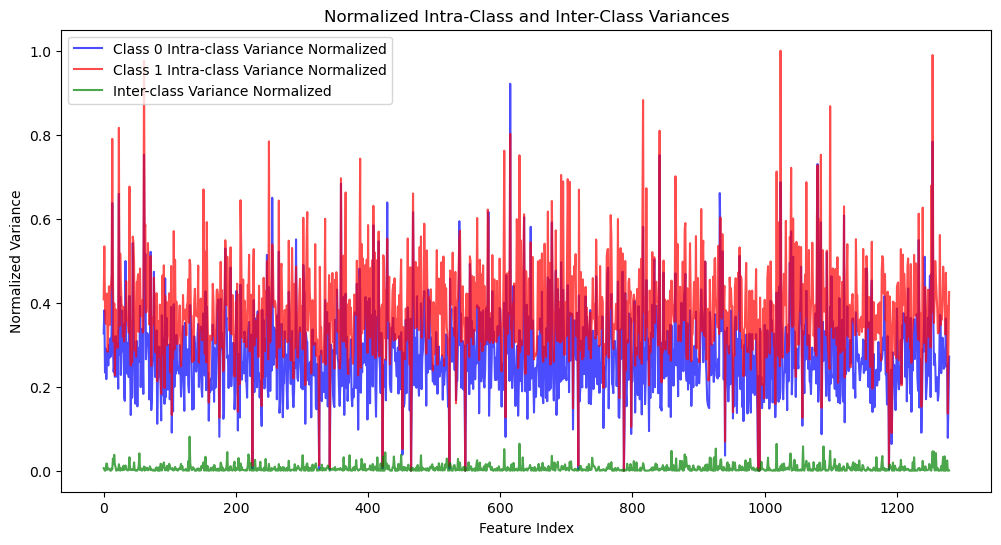
\includegraphics[width=0.8\textwidth]{Images_Thesis/variance_d_b/output_normalized_variance_07.png}
\end{center}
\caption[Feature variance analysis using the vision transformer model.]{Feature variance analysis using the vision transformer model. Displays intra-class variance curves for `non-distracted' (blue) and `distracted' (red) drivers, with the green line depicting inter-class variance. The x-axis denotes the 1280 features extracted, and the y-axis shows normalized variance values, using the highest observed variance of 0.00423 for normalization.}
\label{fig:variance_analysis_image}
\end{figure}

\paragraph{Challenges in Class Separability:}
The analysis indicates a low inter-class variance of approximately 0.01 and a distance of 0.366 between class centers, suggesting the model's limitations in distinct class differentiation. Nonetheless, these limitations are less critical as the model's primary function is to enrich the input for clustering and weighting rather than direct classification. The HDBSCAN algorithm leverages the broad spectrum of extracted features to generate meaningful clusters, which are more valuable than outright class separability for this application.

This strategy enhances training batch diversity, crucial for improving generalization in the subsequent model training. A weighting strategy that assigns lower weights to outliers (0.001) ensures that these atypical features do not disproportionately influence the training process, mitigating potential biases from high intra-class variance.

Overall, while the feature extraction model may not excel in class discrimination, it captures an extensive range of class features essential for effective clustering and weighted sampling, thus addressing challenges in training with imbalanced and complex datasets.

\subsection{Dataloader Comparison}
In addressing the first research question concerning the issue of data imbalance in the DAA dataset, this section evaluates whether unsupervised learning techniques can effectively rectify this imbalance. Previous studies, as outlined in the chapter~\ref{chapter:related_work}, provide various methods to tackle dataset imbalances, each with distinct advantages and limitations. This thesis proposes an unsupervised learning-based data loading strategy termed ``Clustered Feature Weighting,'' aiming to enhance batch balance during data loading for training deep learning models.

\paragraph{Experiment Setup:}
To assess the efficacy of the ``Clustered Feature Weighting'' strategy against traditional data loading methods, where training data is loaded without addressing imbalances, an experimental comparison was conducted. Detailed methodologies are presented in the methodology section; here, we focus exclusively on the experimental results.

\paragraph{Settings for Clustering \& Weighting:}
\begin{itemize}
    \item \textbf{Algorithm}: HDBSCAN
    \item \textbf{Metric}: Batchwise Cosine Distance Matrix
    \item \textbf{Minimum Cluster Size}: 25
    \item \textbf{Minimum Samples (min\_samples)}: 1
    \item \textbf{Cluster Selection Epsilon}: 0
    \item \textbf{Metric Type}: Precomputed
    \item \textbf{Cluster Selection Method}: EOM
    \item \textbf{Allow Single Cluster}: No
    \item \textbf{Sample Weighting}: $\frac{1}{\text{Number of samples in the cluster}}$
    \item \textbf{Outlier Weight}: 0.001
\end{itemize}

\paragraph{Results:}
Figure~\ref{fig:kl_divergence_plot_0_001} illustrates the KL divergence for dataloader comparison. This plot compares the KL divergence between the ideal uniform distribution per batch per category (shown in red) and the distributions achieved by Traditional Dataloader A (blue) and Clustered Feature Weighting Dataloader B (orange). The y-axis represents the KL divergence value, while the x-axis shows the number of batches with a batch size of 1024 for the split 0 train dataset of Kinect Color Right Top Image DAA, containing 259,865 total image samples. A lower KL divergence value indicates a closer approximation to the ideal uniform distribution.

\begin{figure}[h]
\begin{center}
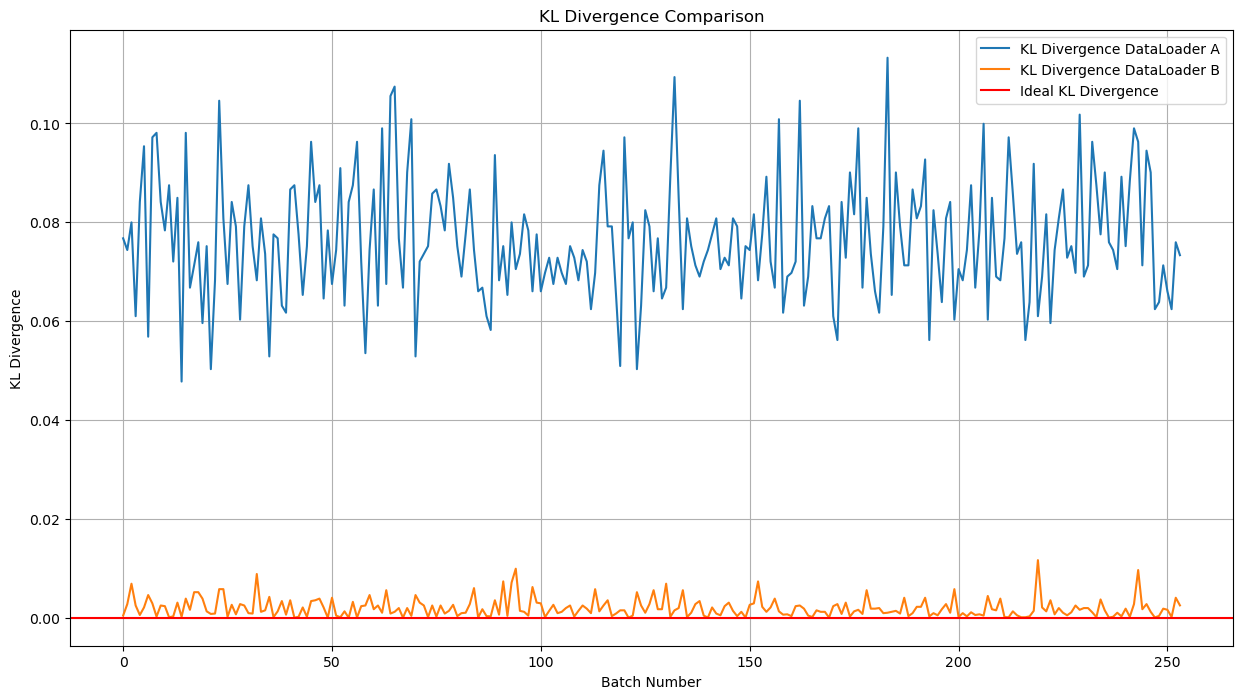
\includegraphics[width=0.8\textwidth]{Images_Thesis/Dataloader_comp/Images_0_001/output_with_uniform_kl_results_grid_0_001.png}
\end{center}
\caption[Comparative KL divergence analysis across multiple batches for dataloading strategies.]{Comparative KL Divergence Analysis Across Multiple Batches for Two Dataloading Strategies. This plot visualizes the KL divergence values on the y-axis against the batch numbers on the x-axis, comparing the uniformity of category distribution per batch between the traditional dataloading approach (Dataloader A, shown in blue) and the novel clustered feature weighting strategy (Dataloader B, shown in orange). The plot demonstrates how closely each strategy approximates the ideal uniform distribution across categories, highlighting the effectiveness of the clustered feature weighting in achieving more balanced data loading.}
\label{fig:kl_divergence_plot_0_001}
\end{figure}

\paragraph{Analysis of KL Divergence Plot:}
\begin{itemize}
    \item \textbf{General Trend}: Both lines on the plot denote the KL divergence for each batch, with Dataloader A depicted in blue and Dataloader B in orange.
    \item \textbf{Dataloader A (Blue Line)}: The values fluctuate around 0.08 and higher, suggesting significant divergence from the uniform distribution. This indicates imbalanced class representation within each batch, particularly with over-representation of the `distracted' driver category.
    \item \textbf{Dataloader B (Orange Line)}: The values generally remain below 0.01, close to the ideal zero, which indicates a more balanced class representation within batches.
\end{itemize}

\paragraph{Interpretation and Assessment:}
\begin{itemize}
    \item \textbf{Balanced Sampling}: Dataloader B's performance, characterized by lower and more stable KL divergence values, demonstrates its effective balanced sampling across categories. This contrasts with Dataloader A, which shows greater batch-to-batch category imbalance.
    \item \textbf{Consistency and Predictability}: Dataloader B exhibits consistent and predictable sampling behavior, essential for stable deep learning training. In contrast, the imbalance observed in Dataloader A could potentially lead to less effective model training and generalization.
    \item \textbf{Suitability for Deep Learning Experiments}: Given the goal of achieving a balanced and unbiased representation of categories in training batches, Dataloader B is preferable for training robust deep learning models. It potentially reduces the risk of overfitting to dominant categories.
\end{itemize}

\begin{figure}[htbp]
    \centering
    % First row
    \begin{subfigure}[b]{0.7\textwidth}
        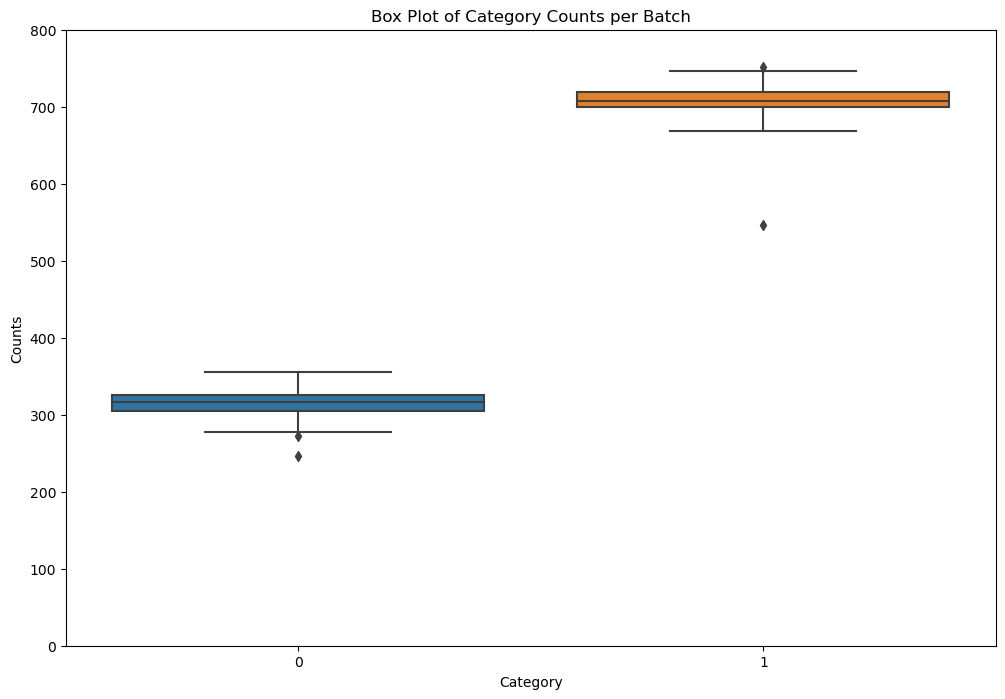
\includegraphics[width=\textwidth]{Images_Thesis/Dataloader_comp/Images_0_001/output_d_a_binary_box_plot_0_001.png}
        \caption{Dataloader A-Traditional Dataloading without Balancing.}
        \label{fig:Box plot for 0_001 experiment with dataloader A}
    \end{subfigure}
    \hfill % space between images
    \begin{subfigure}[b]{0.7\textwidth}
        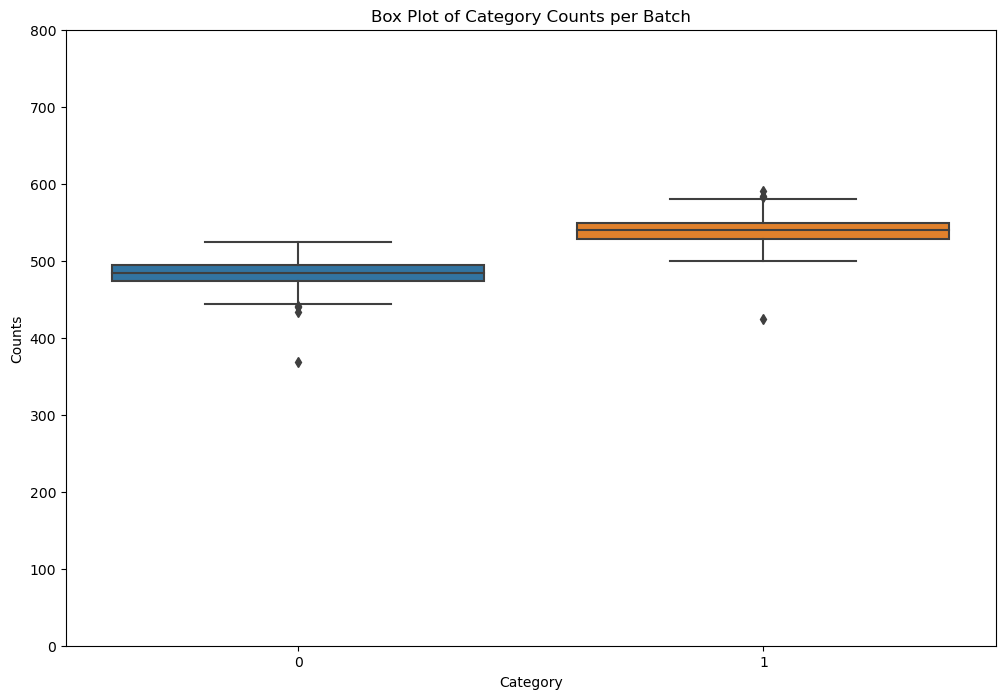
\includegraphics[width=\textwidth]{Images_Thesis/Dataloader_comp/Images_0_001/output_d_b_box_plot_0_001.png}
        \caption{Dataloader B-With Clustered Feature Weighting Strategy for Balancing.}
        \label{fig:Box plot for 0_001 experiment with dataloader B (novel)}
    \end{subfigure}

    \caption[Box plot analysis of sample counts per batch for dataloading strategies.]{Box Plot Analysis of Sample Counts per Batch for Two Dataloading Strategies. This figure displays box plots that illustrate the distribution of sample counts per batch for nondistracted (Category 0) and distracted (Category 1) driver categories, using both (a) Dataloader A and (b) Dataloader B. The box plots show the spread, central tendency, and outliers for each category within the batches. Dataloader B, which employed an outlier weight of 0.001, demonstrates how this parameter influences the balance and uniformity of sample distribution compared to Dataloader A.}
    \label{fig:Box plot dataloader A and dataloader B with 0_001}
\end{figure}

%%%%%%%%%%%%%%%%%% Grid of class distributions %%%%%%%%%%%%%%%%%
\paragraph{Analysis of Category Counts per Batch Using Box Plots:}
Figure~\ref{fig:Box plot dataloader A and dataloader B with 0_001} presents a box plot visualization of the counts of samples per batch for two categories of driver distraction: nondistracted (Category 0) and distracted (Category 1) across two different dataloaders under comparison, A and B. These box plots are instrumental in assessing the balance of sample distribution across categories within each batch.

In Dataloader A, see~\ref{fig:Box plot dataloader A and dataloader B with 0_001}-(a), the median count for Category 0 (non-distracted) is notably lower at approximately 310 counts, whereas for Category 1 (distracted), it is significantly higher at about 710 counts. This discrepancy indicates a skewed distribution in each batch, which could lead to biased model training due to the over-representation of distracted drivers.

Conversely, Dataloader B, see~\ref{fig:Box plot dataloader A and dataloader B with 0_001}-(b), shows a more balanced approach, with the median counts for Category 0 and Category 1 being much closer to each other, around 480 and 530 counts, respectively. These values suggest a more equitable distribution of categories within batches, which is closer to the ideal scenario where each category would ideally comprise half of the batch size of 1024, meaning 512 samples from Category 0 and 512 samples from Category 1. The comparison of these medians between the two dataloaders indicates that Dataloader B is more effective in creating balanced batches.

\paragraph{Impact of Outlier Weight on Sampling:}
The selection of an outlier weight of 0.001 in our experiments was a deliberate decision informed by extensive empirical testing. This parameter was fine-tuned through a systematic trial-and-error process, exploring a range of values from 0 to 1. The impact of the outlier weight on the sampling process is crucial, as it directly influences the KL divergence values, which measure the discrepancy between the actual data distribution in each batch and the ideal uniform distribution across categories.

Figure~\ref{fig:kl_divergence_plot_0_02} illustrates the effects of utilizing a higher outlier weight of 0.02 in Dataloader B. The results indicate a significant increase in the KL divergence values, averaging around 0.07, which suggests a deviation from the ideal uniform distribution. This deviation is substantiated by the increased KL divergence, highlighting the sensitivity of the sampling process to the outlier weight setting.

Moreover, the corresponding box plots in Figure~\ref{fig:Box plot for 0_02 experiment with dataloader B (novel)} for categories 0 and 1 reveal a noticeable difference between the medians of counts of each category. This difference underscores a pronounced imbalance in the batch compositions of Dataloader B when a higher outlier weight is employed. The divergence of the medians from each other at this higher outlier weight (0.2) confirms that the distribution of samples across categories becomes significantly skewed, detracting from the efficacy of the dataloading process in maintaining balanced batches.

\begin{figure}[htbp]
\begin{center}
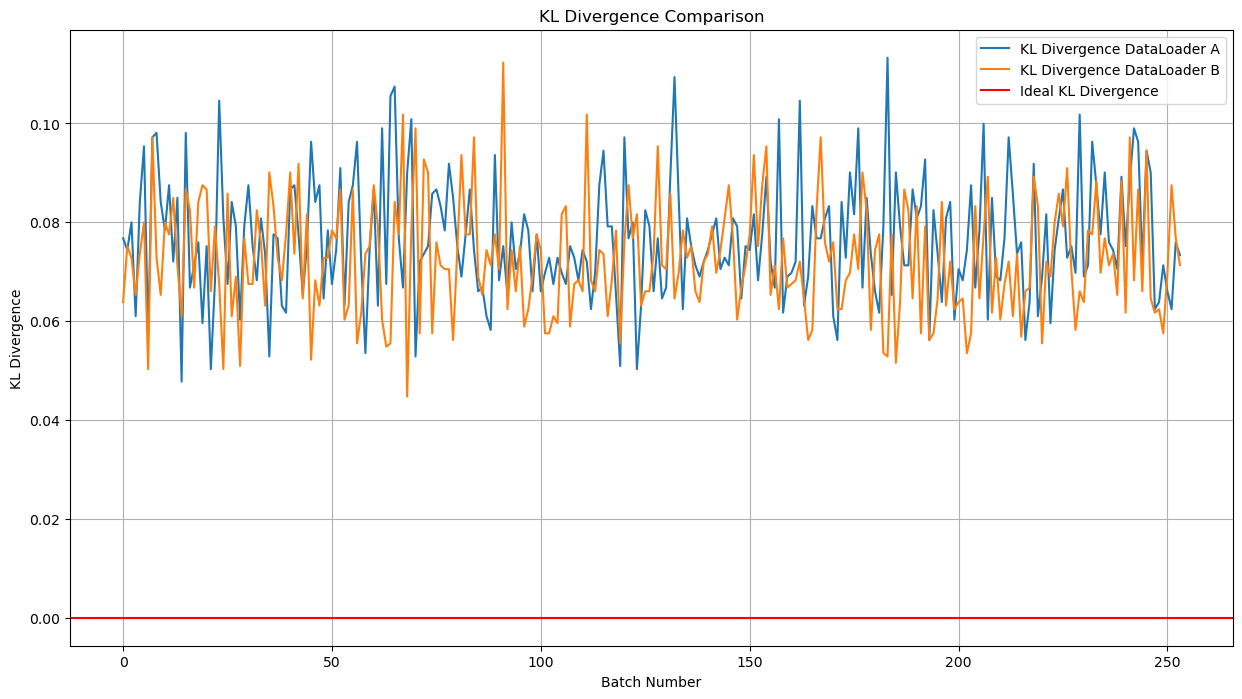
\includegraphics[width=0.8\textwidth]{Images_Thesis/Dataloader_comp/Images_0_02/output_0_02_outlier_weight_KL.png}
\end{center}
\caption[KL divergence analysis with increased outlier weight.]{KL Divergence Analysis with Increased Outlier Weight. This plot displays the KL divergence values on the y-axis versus the number of batches on the x-axis, comparing the traditional dataloading approach (Dataloader A) and the novel clustered feature weighting strategy (Dataloader B), evaluated with an outlier weight of 0.02. The divergence from the ideal uniform distribution across categories per batch is indicated, with Dataloader B (shown in orange) and Dataloader A (shown in blue), highlighting how the increased outlier weight affects the effectiveness of each dataloading strategy in achieving category balance.}
\label{fig:kl_divergence_plot_0_02}
\end{figure}

%%%%%%%%%%%%%%%%%% Grid of class distributions %%%%%%%%%%%%%%%%%
\begin{figure}[htbp]
    \centering
    % First row
    \begin{subfigure}[b]{0.7\textwidth}
        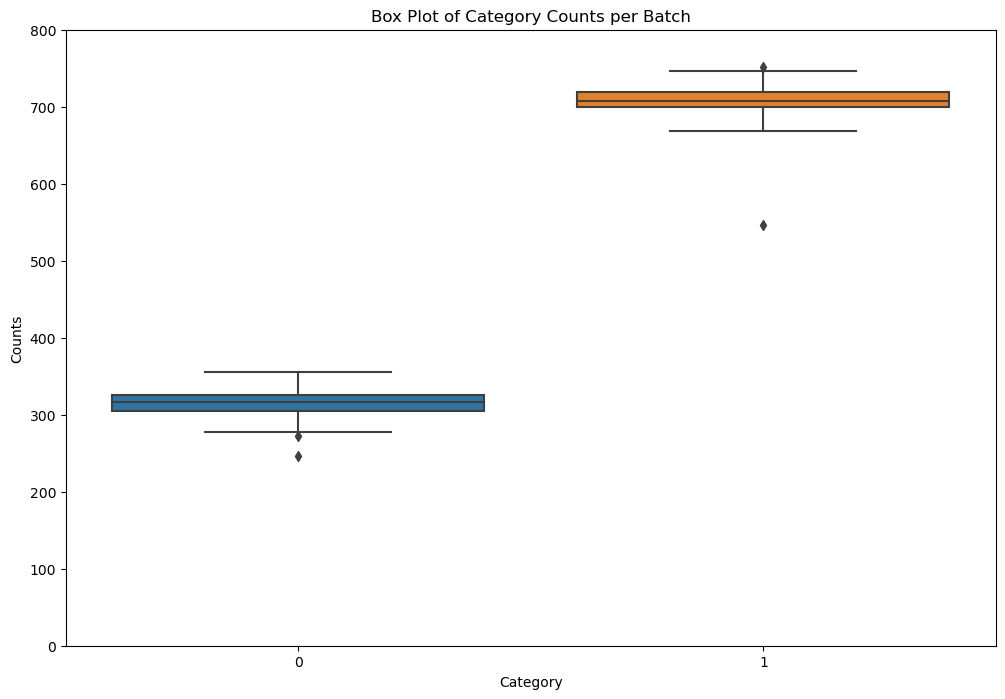
\includegraphics[width=\textwidth]{Images_Thesis/Dataloader_comp/Images_0_02/output_box_0_02_d_a.png}
        \caption{Dataloader A- Traditional Dataloading without Balancing.}
        \label{fig:Box plot for 0_02 experiment with dataloader A}
    \end{subfigure}
    \hfill % space between images
    \begin{subfigure}[b]{0.7\textwidth}
        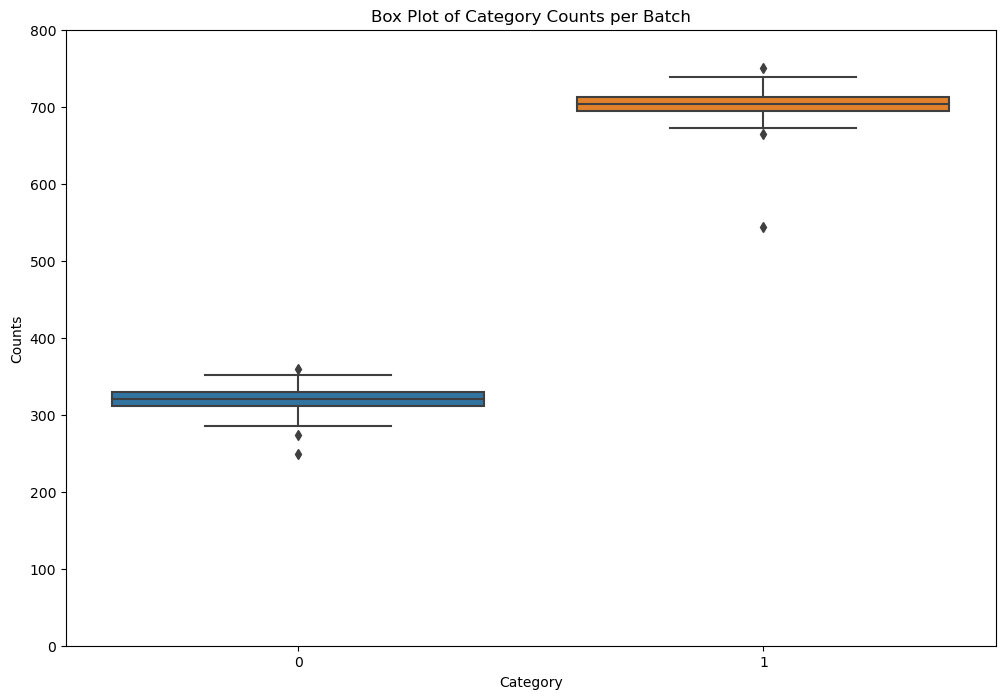
\includegraphics[width=\textwidth]{Images_Thesis/Dataloader_comp/Images_0_02/output_KL_0_02_d_b.png}
        \caption{Dataloader B- With Clustered Feature Weighting Strategy for Balancing.}
        \label{fig:Box plot for 0_02 experiment with dataloader B (novel)}
    \end{subfigure}

    \caption[Box Plot Analysis of Category Counts per Batch with an Increased Outlier Weight for Dataloader B.]{ Box Plot Analysis of Category Counts per Batch with an Increased Outlier Weight for Dataloader B. This figure presents box plots depicting the distribution of sample counts per batch for nondistracted (Category 0) and distracted (Category 1) driver categories, utilizing both Dataloader A and Dataloader B. These plots illustrate the spread, central tendency, and identification of outliers within each category's distribution across batches. Notably, Dataloader B is evaluated using an increased outlier weight of 0.02, highlighting the impact of this weight adjustment on the balance and uniformity of sample distribution compared to Dataloader A.}
    \label{fig:Box plot dataloader A and dataloader B with 0_02}
\end{figure}

\paragraph{Dataloader Experiments Conclusion:}
The comprehensive evaluation of dataloaders in this study highlights the superior performance of Dataloader B, which utilizes a clustered feature weighting strategy proposed in this thesis. This strategy significantly improves the data imbalance in training deep learning models, as demonstrated by the KL divergence and box plot analyses.

Dataloader B consistently achieved lower KL divergence values, indicating a more uniform distribution that aligns closely with the ideal uniform distribution across categories per batch. Additionally, the box plot analysis~\ref{fig:Box plot dataloader A and dataloader B with 0_001} confirmed that Dataloader B provides a more balanced distribution of both `non-distracted' and `distracted' categories within each batch. The median counts of these categories are nearly even, closely approaching the ideal split of the batch size.

In conclusion, Dataloader B ensures a more equitable representation of categories. However, this proposed novel data loading strategy still needs a verification for gain in model learning and generalisation compared to traditional dataloading.

\section{Experiments based on Model Training and Evaluation}
\subsection{Hyperparameter Grid Search Results}
A rigorous hyperparameter search was conducted using a 10\% subset of the split 0 of Kinect Color Image DAA dataset, sampled through stratified sampling method to reflect the inherent imbalance of the split 0 of the Kinect Color image DAA dataset. This process aimed to optimize model performance by identifying the most effective hyperparameters for this specific context.~\citet{Vit_Paper_Dosovitskiy2020AnII} recommended the Stochastic Gradient Descent (SGD)~\citep{pytorch_sgd} optimizer for transfer learning on vision transformer models due to its suitability in handling pretrained architectures.

The primary objective of the hyperparameter grid search was to ascertain the optimal learning rate and validate the superiority of SGD over Adam~\citep{Adam_Kingma2014AdamAM} for fine-tuning linear layer on top of frozen pre-trained vision transformers on the Kinect Color Right Top DAA dataset. Key elements of the initial setup included:
\begin{itemize}
    \item \textbf{Learning Rate Sweep:} A systematic exploration of learning rates—0.003, 0.01, 0.03, 0.06—is conducted to determine the optimal rate for training the linear layer atop the frozen encoder, gauged over 20,000 steps using validation set performance.
    \item \textbf{Steps and Epochs Calculation:} Given the 259,865 images in the train dataset of split 0 of the Kinect Color DAA Image dataset and a batch size of 1024, it takes 254 steps to complete one epoch. To achieve 20,000 steps, approximately 79 epochs are necessary. Consequently, all experiments are extended to 100 epochs to ensure adequate model convergence.
    \item \textbf{Additional Parameters:} The search also included fine-tuning parameters such as a momentum of 0.9, no weight decay, and gradient clipping at a global norm of 1 as used in the~\citep{Vit_Paper_Dosovitskiy2020AnII} for fine tuning. The resolution for fine-tuning was set at 224 pixels.
\end{itemize}

To ensure stable training conditions, the hyperparameter search was expanded to include various learning rate schedulers like Linear Decay, Step Decay, Exponential Decay, and Constant LR, alongside necessary adjustments for each strategy. Appendix section provides more details about the results of these experiments.

Experiment results, as shown in Table \ref{table:top-competitors}, indicate that training balanced accuracies are consistently high (greater than 92\%), whereas validation balanced accuracies are considerably lower (83.45\% to 83.87\%), suggesting a potential overfitting issue. Notably, the learning rate adjustments between experiments varied, with Experiment 22 starting at $4.00 \times 10^{-4}$ and reducing to $2.00 \times 10^{-4}$, and Experiment 23 implementing a higher initial rate that decreased more significantly to $1.00 \times 10^{-4}$. These configurations resulted in the smallest gaps between training and validation accuracies (8.18\% and 8.17\%, respectively), indicating better generalization compared to Experiment 25, which had a larger gap of 9.18\%. These findings underscore the importance of finely tuned learning rate schedules in balancing between achieving high training accuracy and ensuring good generalization to unseen data.

Using the Adam optimizer with cosine annealing significantly lowered performance in terms of validation accuracy; however, utilizing Adam with a linear decay scheduler, as depicted in Experiment 24 in appendix section in Table ~\ref{table:lineadecay-detailed}, yielded a validation balanced accuracy of 80.86\%, with a pronounced discrepancy of 15.80\% between training and validation accuracies. In total, 16 experiments combining the Adam and SGD optimizers with the Cosine Annealing scheduler were conducted. The maximum number of iterations (\(T_{\text{max}}\)) set for the cosine annealing was 100 and 10, as shown in the appendix section in Table~\ref{table:cosineannealing-tmax}. These experiments consistently resulted in a balanced accuracy gap exceeding 10\%, indicative of substantial overfitting. Based on the hyperparameter settings and experiments conducting using Adam and SGD optimizer, SGD optimizer performed better than Adam optimizer which aligns with the choice of~\citep{Vit_Paper_Dosovitskiy2020AnII} for fine tuning vision transformer on downstream tasks like image classification on custom datasets.

Further analysis involving the SGD optimizer paired with a Linear Decay scheduler and varying initial and final learning rates, detailed in appendix section in Table~\ref{table:lineadecay-detailed}, revealed that configurations with lower starting and ending rates effectively decreased the overfitting issue. Similarly, using the Step Decay scheduler with a decay factor of 0.1 every 20 epochs also led to overfitting, with a gap exceeding 10\%. This pattern persisted in four experiments utilizing an Exponential Decay scheduler with the SGD optimizer, refer to appendix section in Table~\ref{table:exponentialdecay-performance}, each also exhibiting significant overfitting. To assess the impact of a constant learning rate on overfitting, two additional experiments were conducted with learning rates of 0.001 and 0.003, refer to appendix section in Table ~\ref{table:constantlr-performance}, resulting in gaps of 13.70\% and 14.64\%, respectively, and validation accuracies of 81.07\% and 81.39\%.

Considering these outcomes, the hyperparameter settings from Experiment 22, which demonstrated a smaller gap between training and validation balanced accuracies, are adopted as the baseline for main experiments, as illustrated in the table~\ref{table:chosen hyperparameter configurations}.

\begin{table}[ht]
\caption{Chosen hyperparameter configurations}
\label{table:chosen hyperparameter configurations}
\centering
\begin{tabular}{ll}
\multicolumn{1}{c}{\textbf{PARAMETER}} & \multicolumn{1}{c}{\textbf{VALUE}} \\
\hline
Experiment Number & 22 \\
Epochs & 100 \\
Effective Batch Size & 1024 \\
Number of GPUs & 2 \\
Batch Size per GPU & 512 \\
Optimizer & SGD \\
Scheduler & LinearDecay \\
Initial LR & $4.00 \times 10^{-4}$ \\
End LR & $2.00 \times 10^{-4}$ \\
Train Balanced Accuracy & 92.05\% \\
Validation Balanced Accuracy & 83.87\% \\
Balanced Accuracy Gap & 8.18\% \\
\hline
\end{tabular}
\end{table}

\begin{table}[ht]
\caption{Top competing hyperparameter configurations}
\label{table:top-competitors}
\centering
\small
\begin{tabular}{llllll}
\multicolumn{2}{c}{\textbf{Experiment Details}} & \multicolumn{1}{c}{\textbf{Learning Rate}} & \multicolumn{3}{c}{\textbf{Balanced Accuracy}} \\
\hline
\textbf{Exp No} & \textbf{Optimizer-Scheduler} & \textbf{Initial LR - End LR} & \textbf{Train} & \textbf{Validation} & \textbf{Gap} \\
\hline
22 & SGD - LinearDecay & $4.00 \times 10^{-4} - 2.00 \times 10^{-4}$ & 92.05\% & 83.87\% & 8.18\% \\
23 & SGD - LinearDecay & $5.00 \times 10^{-4} - 1.00 \times 10^{-4}$ & 92.00\% & 83.83\% & 8.17\% \\
25 & SGD - LinearDecay & $4.50 \times 10^{-4} - 1.50 \times 10^{-4}$ & 92.62\% & 83.45\% & 9.18\% \\
\hline
\end{tabular}
\end{table}

\begin{figure}[htbp]
\begin{center}
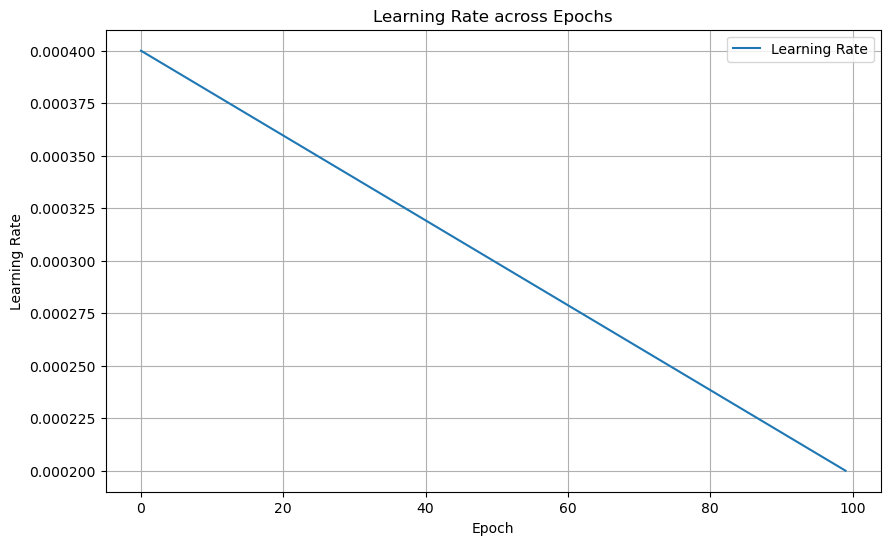
\includegraphics[width=0.8\textwidth]{Images_Thesis/Tensboard_runs_images_all/Experiment_00_Sup_D_A_no_Aug/Split_0/output_learningrate.png}
\end{center}
\caption[Linear learning rate decay used in all four experiments.]{Linear learning rate decay: the learning rate schedule starts at initial learning rate of 0.0004 and ends at 0.0002 after 100 epochs. The epochs on the x-axis are 0 indexed.}
\label{fig:learning rate plot}
\end{figure}

%%%%%%%%%%%%%%%%%%%%%%%%%%%%%%%%%%%%%%%%%%%%%%%%%%%%%%%%%%%%%%
%%%%%%%%%%%%%%%%%%%%%%%%%%%%%%%%%%%%%%%%%%%%%%%%%%%%%%%%%%%%%%
%%%%%%%%%%%%%%%%%%%%%%%%%%%%%%%%%%%%%%%%%%%%%%%%%%%%%%%%%%%%%%
\subsection{Results of Experiment 1: Supervised Learning Based Encoder}
%%%%%%%%%%%%%%%%%%%%%%%%%%%%%%%%%%%%%%%%%%%%%%%%%%%%%%%%%%%%%%
Following the methodology explained in section~\ref{section:Methodology Experiment 1: Supervised Learning Based Encoder}, in this experiment, we adapted a pre-trained Vision Transformer (vit\_b\_16) model, pre-trained on the ImageNet-1K dataset, for the driver distraction detection task using the Kinect Color Right Top view dataset. We replaced the (vit\_b\_16) classifier layer with a linear layer, training only this component to leverage the model's transfer learning and feature extraction capabilities. The hyperparameters selected in the previous section played a crucial role in training our model. These included a linear decay scheduler for the learning rate, starting at $4.00 \times 10^{-4}$ and decreasing to $2.00 \times 10^{-4}$ over 100 epochs, as illustrated in Figure~\ref{fig:learning rate plot}. The model was trained with an effective batch size of 1024, distributed across two GPUs using the Distributed Data-Parallel (DDP) algorithm. The results of this experiment are presented in Table~\ref{table:experiment 1 results}.
%%%%%%%%%%%%%%%%%% Grid of Plots %%%%%%%%%%%%%%%%%
\begin{figure}[htbp]
    \centering
    % First row
    \begin{subfigure}[b]{0.45\textwidth}
        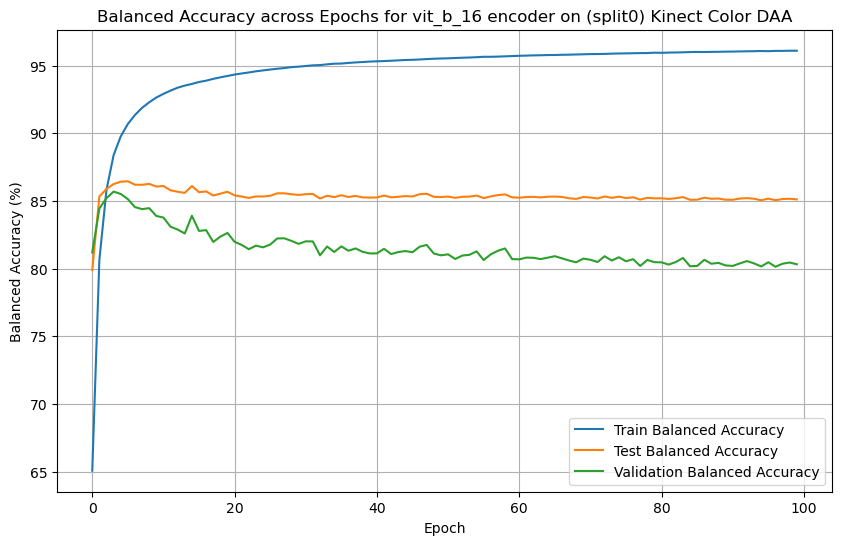
\includegraphics[width=\textwidth]{Images_Thesis/Tensboard_runs_images_all/Experiment_00_Sup_D_A_no_Aug/Split_0/output_bal_acc_no_aug.png}
        \caption{Split 0: Balanced Accuracy vs Epochs}
        \label{fig:Exp_1_01}
    \end{subfigure}
    \hfill % space between images
    \begin{subfigure}[b]{0.45\textwidth}
        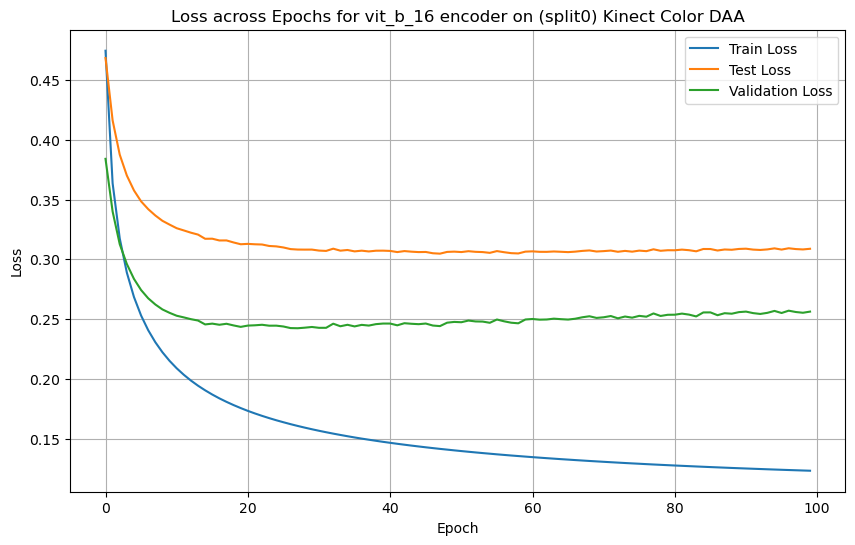
\includegraphics[width=\textwidth]{Images_Thesis/Tensboard_runs_images_all/Experiment_00_Sup_D_A_no_Aug/Split_0/output_loss_splt_0_no_aug_d_a.png}
        \caption{Split 0: Loss vs Epochs}
        \label{fig:Exp_1_02}
    \end{subfigure}

    % Second row
    \begin{subfigure}[b]{0.45\textwidth}
        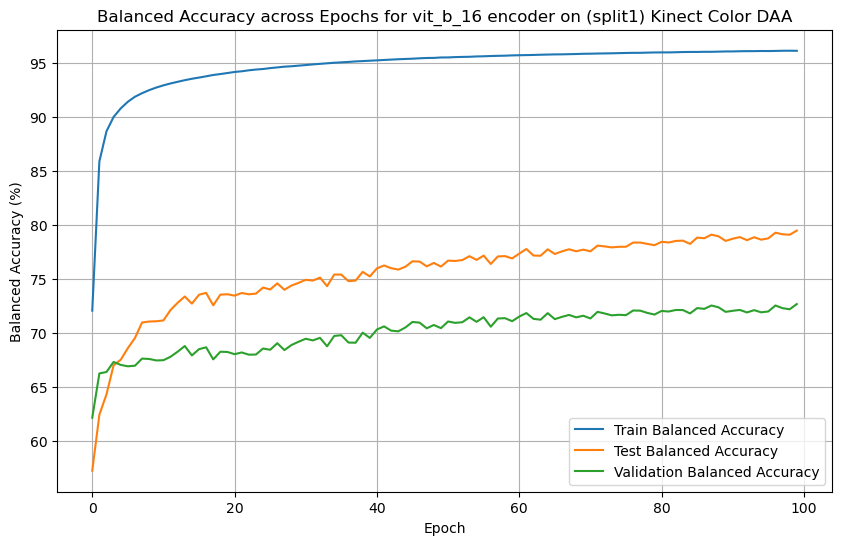
\includegraphics[width=\textwidth]{Images_Thesis/Tensboard_runs_images_all/Experiment_00_Sup_D_A_no_Aug/Split_1/output_bal_acc_d_a_no_aug.png}
        \caption{Split 1: Balanced Accuracy vs Epochs}
        \label{fig:Exp_1_03}
    \end{subfigure}
    \hfill
    \begin{subfigure}[b]{0.45\textwidth}
        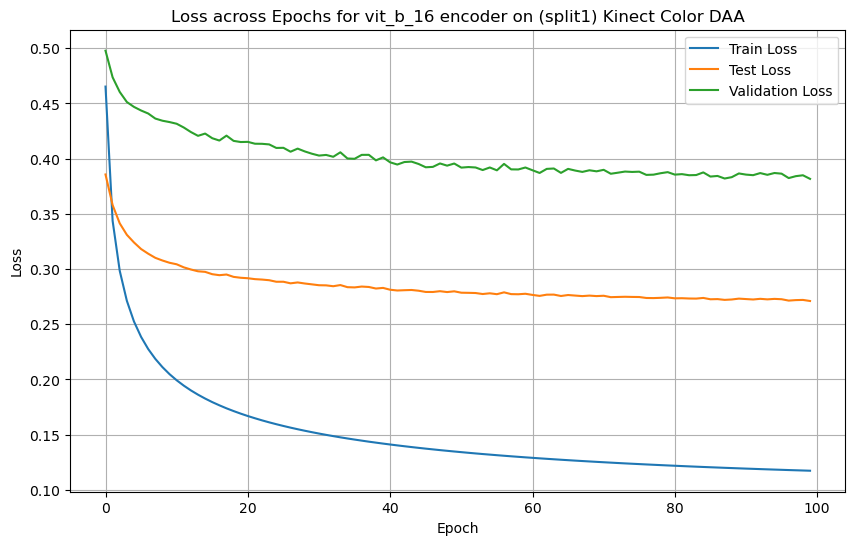
\includegraphics[width=\textwidth]{Images_Thesis/Tensboard_runs_images_all/Experiment_00_Sup_D_A_no_Aug/Split_1/output_loss_d_a_no_aug_split_1.png}
        \caption{Split 1:  Loss vs Epochs}
        \label{fig:Exp_1_04}
    \end{subfigure}

    % Third row
    \begin{subfigure}[b]{0.45\textwidth}
        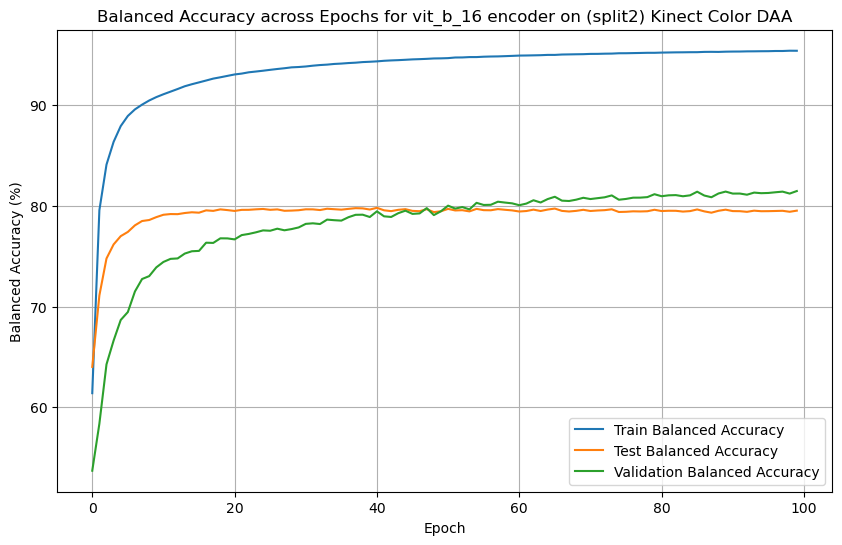
\includegraphics[width=\textwidth]{Images_Thesis/Tensboard_runs_images_all/Experiment_00_Sup_D_A_no_Aug/Split_2/output_bal_acc_split_2_d_a_no_aug.png}
        \caption{Split 2: Balanced Accuracy vs Epochs}
        \label{fig:Exp_1_05}
    \end{subfigure}
    \hfill
    \begin{subfigure}[b]{0.45\textwidth}
        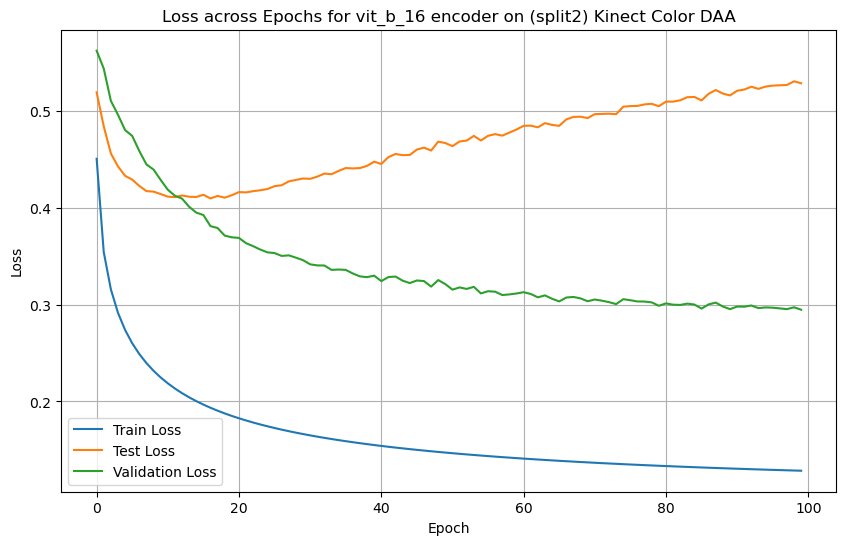
\includegraphics[width=\textwidth]{Images_Thesis/Tensboard_runs_images_all/Experiment_00_Sup_D_A_no_Aug/Split_2/output_loss_split_2_d_a_no_aug.png}
        \caption{Split 2: Loss vs Epochs}
        \label{fig:Exp_1_06}
    \end{subfigure}
    \caption[Results of Experiment 1: Supervised Learning Based Encoder]{Comparison of training and evaluation based on balanced accuracy an loss curves plotted across epochs for all three splits of Kinect Color Right Top view DAA Image dataset for supervised learning based encoder in experiment 1.}
    \label{fig:Exp_1_00}
\end{figure}

The average training balanced accuracy across all splits is notably high at 95.88\%, demonstrating the model's robust ability to learn from the training data. However, the validation balanced accuracies are considerably lower, averaging 78.16\%, which indicates overfitting. The average test accuracy is somewhat higher at 81.38\%, indicating a reasonable generalization to unseen data.

Validation-balanced accuracies are much lower than training-balanced accuracies, indicating that the model struggles to generalize across dataset subsets. This discrepancy may be due to the unique Kinect Color Right Top view image dataset or limits in the transferability of pre-trained features to driver distraction detection task and requires further research in this direction. Similarly, the significant difference between training and validation balanced accuracy in Table~\ref{table:experiment 1 results}, especially in Split 1, shows overfitting. 
%%%%%%%%%%%% Result table: Experiment 1 %%%%%%%%%%%
\begin{table}[htbp]
\caption[Results of experiment 1: supervised learning based encoder]{Supervised learning based encoder results on driver distraction detection task. The linear layer on top of pretrained frozen encoder (vit\_b\_16) is trained and evaluated on all three splits of Kinect Color Right Top DAA image dataset for 100 epochs using DDP algorithm on dual GPU setup with an effective batch of 1024. The results are avearged for 100th epoch for comparison with subsequent experiments.}
\label{table:experiment 1 results}
\centering
\begin{tabular}{lllllll}
\multicolumn{1}{c}{\textbf{Splits}} & \multicolumn{1}{c}{\textbf{View}} & \multicolumn{1}{c}{\textbf{Encoder}} & \multicolumn{1}{c}{\textbf{Epoch}} & \multicolumn{1}{c}{\textbf{Train}} & \multicolumn{1}{c}{\textbf{Val}} & \multicolumn{1}{c}{\textbf{Test}}\\
\hline
Split\_0 & Right Top & vit\_b\_16 & 100 & 96.10\% & 80.32\% & 85.12\% \\
Split\_1 & Right Top & vit\_b\_16 & 100 & 96.12\% & 72.69\% & 79.49\% \\
Split\_2 & Right Top & vit\_b\_16 & 100 & 95.42\% & 81.48\% & 79.53\% \\
\hline
Average & Right Top & vit\_b\_16 & 100 & 95.88\% & 78.16\% & 81.38\% \\
\hline
\end{tabular}
\end{table}

Figure~\ref{fig:Exp_1_00} shows this experiment's balanced accuracy and loss curves. It can be seen in the figure that each split exhibits high initial training balanced accuracies, quickly reaching a plateau. This behavior underscores the effective utilization of the pre-trained features of the ViT-B/16, which is adept at adapting quickly to the training data. However, the validation and test accuracies across the splits show varied patterns. Test-balanced accuracies generally stabilize at higher levels than validation, suggesting better generalization on the test set. Notably, Split 2 shows a closer convergence between validation and test balanced accuracies, indicating more effective generalization compared to Splits 0 and 1.

Similarly, the loss curves in the figure~\ref{fig:Exp_1_00} show sharp initial declines in training loss in all splits, reflecting efficient error minimization on training data. However, the validation loss behaviors vary, with Split 2 displaying an increasing trend after initial stabilization—signaling potential overfitting or inadequate model tuning for generalization.

The trained linear layer on top of the frozen supervised learning-based encoder (vit\_b\_16) in this experiment is further tested for cross-modality and cross-view generalization on the Kinect IR and NIR DAA test datasets across all splits, as described in sections~\ref{section:Methodology for Cross-Modality Generalization Evaluation} and~\ref{section:Methodology for Cross-View Generalization Evaluation}. Tables \ref{table:experiment 1 results Cross Modality Generalisation} and \ref{table:experiment 1 results Cross Modality and view Generalisation on NIR} shows the model's performance on Kinect IR and NIR DAA image datasets with different camera view and image modality than the training dataset.

%%% Cross Modality Generalisation Tables %%%%%%%%%%
\begin{table}[htbp]
\caption[Results of Experiment 1 for Cross Modality Generalisation]{Performance of the Linear Layer trained on top of the Frozen Supervised Encoder on Kinect IR Right Top View Dataset: This table shows the results from evaluating the 100th checkpoint of the model, initially trained on color images, on the grayscale test sets of the Kinect IR Right Top view dataset.}
\label{table:experiment 1 results Cross Modality Generalisation}
\centering
\begin{tabular}{lllll}
\multicolumn{1}{c}{\textbf{Splits}} & \multicolumn{1}{c}{\textbf{View}} & \multicolumn{1}{c}{\textbf{Encoder}} & \multicolumn{1}{c}{\textbf{Checkpoint}} & \multicolumn{1}{c}{\textbf{Test}}\\
\hline
Split\_0 & Right Top & vit\_b\_16 & 100 & 49.96\% \\
Split\_1 & Right Top & vit\_b\_16 & 100 & 57.83\% \\
Split\_2 & Right Top & vit\_b\_16 & 100 & 52.42\% \\
\hline
Average & KIR Right Top & vit\_b\_16 & 100 & 53.40\% \\
\hline
\end{tabular}
\end{table}

\textbf{Cross-Modality and Cross-View Generalization:}
The performance on the Kinect IR Right Top view dataset (Table \ref{table:experiment 1 results Cross Modality Generalisation}) shows that the model achieves an average test balanced accuracy of 53.40\%. This result is considerably lower than the training balanced accuracies observed on the Kincet Color DAA dataset, highlighting challenges in the model's ability to generalize to grayscale IR images. Individual splits show variability, with the highest being 57.83\% in Split 1 and the lowest at 49.96\% in Split 0, suggesting some inconsistency in the model's performance across different segments of the Kinect IR dataset.

Further evaluating the model's generalization capabilities, the NIR Front Top view dataset (Table \ref{table:experiment 1 results Cross Modality and view Generalisation on NIR}) shows even more uniform results with a narrow range of test balanced accuracies hovering around 49\%. The average balanced accuracy across the splits stands at 49.24\%, which is slightly lower than the Kinect IR dataset results. This indicates additional challenges when the model encounters not only a different modality but also a different viewing angle, emphasizing the specificity of the learned features to the training conditions.
%%% Cross Modality & Cross View Generalisation Tables %%%%%%%%%%
\begin{table}[htbp]
\caption[Results of Experiment 1 for Cross Modality and Cross view Generalisation.]{Performance of the Linear Layer trained on top of the Frozen Supervised Encoder on NIR Front Top View DAA Dataset: This table shows the results from evaluating the 100th checkpoint of the model, initially trained on color images, on the grayscale test sets of the NIR Front Top view dataset. Here model evaluation is performed on gray scale images and front top view resulting in cross-modality and cross-view generalization evaluation.}
\label{table:experiment 1 results Cross Modality and view Generalisation on NIR}
\centering
\begin{tabular}{lllll}
\multicolumn{1}{c}{\textbf{Splits}} & \multicolumn{1}{c}{\textbf{View}} & \multicolumn{1}{c}{\textbf{Encoder}} & \multicolumn{1}{c}{\textbf{Checkpoint}} & \multicolumn{1}{c}{\textbf{Test}}\\
\hline
Split\_0 & Front Top & vit\_b\_16 & 100 & 49.79\% \\
Split\_1 & Front Top & vit\_b\_16 & 100 & 49.53\% \\
Split\_2 & Front Top & vit\_b\_16 & 100 & 48.41\% \\
\hline
Average & NIR Front Top & vit\_b\_16 & 100 & 49.24\% \\
\hline
\end{tabular}
\end{table}

These results demonstrate the limitations of applying models trained on specific datasets and modalities to other dataset without adaptation or training. The model's feature extraction abilities appear to be highly related to the training data's features, as color to grayscale images and viewing perspectives significantly decrease performance. Domain adaptation, fine-tuning on target domain datasets, and more diversified training data including many modalities and perspectives may improve cross-modality and cross-view generalization. 

In conclusion, while the linear layer trained on top of frozen encoder vit\_b\_16 demonstrates robust learning capabilities within its training data modality, its application to significantly different data modality without prior adaptation highlights the critical need for models that better generalize across diverse input conditions. Further research into transfer learning and domain generalization techniques would be beneficial to address these challenges and improve the practical utility of such models in real-world applications like driver distraction detection.
%%%%%%%%%%%%%%%%%%%%%%%%%%%%%%%%%%%%%%%%%%%%%%%%%%%%%%%%%%%%%%
\subsection{Results of Experiment 2: Supervised Learning Based Encoder with Gray scale Augmentation}
The results of previous experiment show that without prior training on grayscale image data, the linear layer trained on top of a frozen supervised learning-based encoder (vit\_b\_16) does not generalize effectively on cross-modality and cross-view dataset images. This experiment uses the approach described in section~\ref{section:Methodology 2 Experiment 2: Supervised Learning Based Encoder with Gray scale Augmentation} to assess the model's generalization capabilities while providing grayscale transforms during training. This experiment employed the same training setup as experiment 1, with the main variation being that grayscale transforms were applied to the images fed into the model training. In other words, the color images in the Kinect Color Right Top view dataset are first transformed to grayscale before being given into the model for further training of the linear layer on top of the (vit\_b\_16) encoder. Table~\ref{table:experiment 2 results} summarizes the findings of this experiment.
%%%%%%%%%%%% Result table: Experiment 2 %%%%%%%%%%%
\begin{table}[htbp]
\caption{Results of Experiment 2: Supervised Learning Based Encoder with Gray scale augmentation}
\label{table:experiment 2 results}
\centering
\begin{tabular}{lllllll}
\multicolumn{1}{c}{\textbf{Splits}} & \multicolumn{1}{c}{\textbf{View}} & \multicolumn{1}{c}{\textbf{Augmentation}} & \multicolumn{1}{c}{\textbf{Encoder}} & \multicolumn{1}{c}{\textbf{Train}} & \multicolumn{1}{c}{\textbf{Val}} & \multicolumn{1}{c}{\textbf{Test}}\\
\hline
Split\_0 & Right Top & Gray Scale & vit\_b\_16 & 95.61\% & 68.43\% & 62.25\% \\
Split\_1 & Right Top & Gray Scale & vit\_b\_16 & 95.88\% & 64.28\% & 86.64\% \\
Split\_2 & Right Top & Gray Scale & vit\_b\_16 & 95.12\% & 87.73\% & 84.52\% \\
\hline
Average & Right Top & Gray Scale & vit\_b\_16 & 95.53\% & 73.48\% & 77.80\% \\
\hline
\end{tabular}
\end{table}

Table~\ref{table:experiment 2 results} shows a high average training balanced accuracy of 95.53\% across all splits, indicating the model's strong capacity to learn from augmented grayscale training data. However, the validation balanced accuracies are significantly lower, averaging 73.48 percent, indicating overfitting. The average test balanced accuracy is slightly better at 77.80\%, demonstrating a decent generalization to unseen augmented grayscale data. 

Validation-balanced accuracies are much lower than training-balanced accuracies, indicating that the model trained using grayscale augmentations struggles to generalize across dataset subsets except for split 2, where the validation-balanced accuracy, at 87.73\%, is slightly better than the other two splits. Similarly, the test-balanced accuracy for split 1 and split 2 are much higher than those for split 0.

%%%%%%%%%%%%%%%%%% Grid of class distributions %%%%%%%%%%%%%%%%%
\begin{figure}[htbp]
    \centering
    % First row
    \begin{subfigure}[b]{0.45\textwidth}
        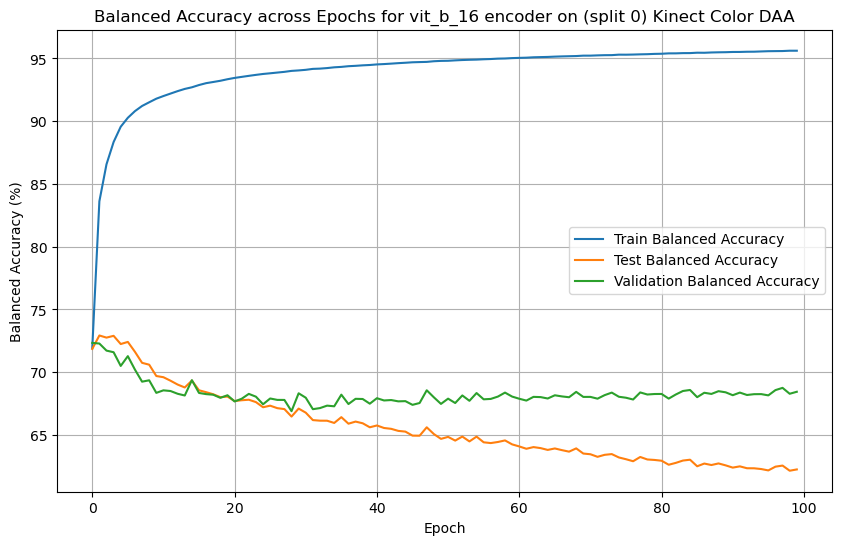
\includegraphics[width=\textwidth]{Images_Thesis/Tensboard_runs_images_all/Experiment_01_Sup_D_A_with_Aug/Split_0/output_bal_acc_split_0_with_aug_d_a.png}
        \caption{Split 0: Balanced Accuracy vs Epochs}
        \label{fig:Exp_2_01}
    \end{subfigure}
    \hfill % space between images
    \begin{subfigure}[b]{0.45\textwidth}
        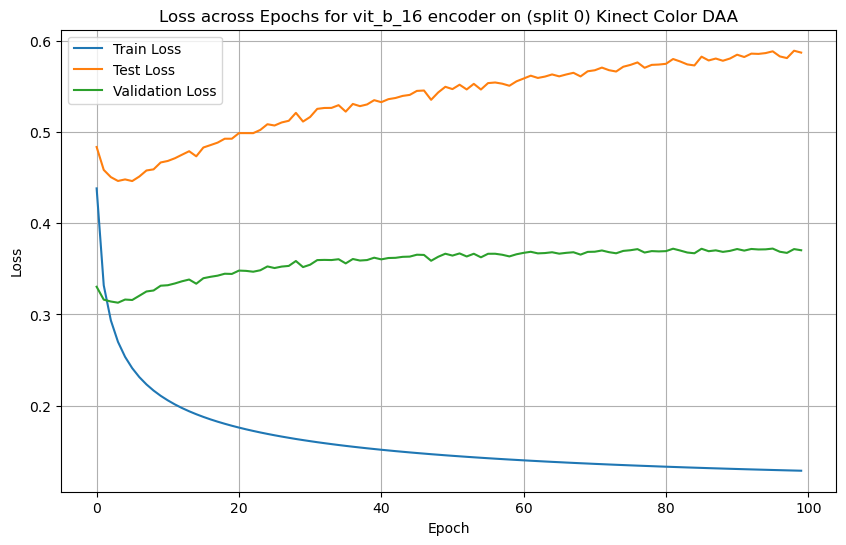
\includegraphics[width=\textwidth]{Images_Thesis/Tensboard_runs_images_all/Experiment_01_Sup_D_A_with_Aug/Split_0/output_loss_split_0_with_aug_d_a.png}
        \caption{Split 0: Loss vs Epochs}
        \label{fig:Exp_2_02}
    \end{subfigure}

    % Second row
    \begin{subfigure}[b]{0.45\textwidth}
        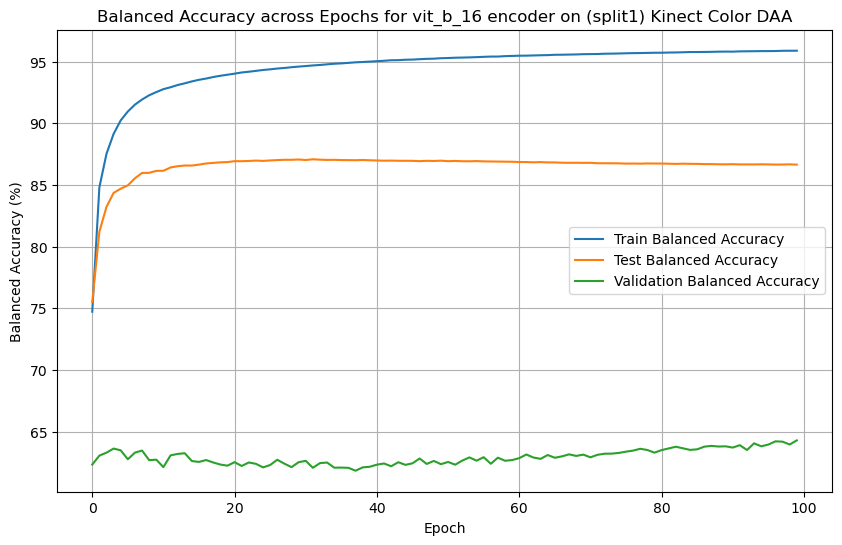
\includegraphics[width=\textwidth]{Images_Thesis/Tensboard_runs_images_all/Experiment_01_Sup_D_A_with_Aug/Split_1/output_bal_acc_split_1_with_aug_d_a.png}
        \caption{Split 1: Balanced Accuracy vs Epochs}
        \label{fig:Exp_2_03}
    \end{subfigure}
    \hfill
    \begin{subfigure}[b]{0.45\textwidth}
        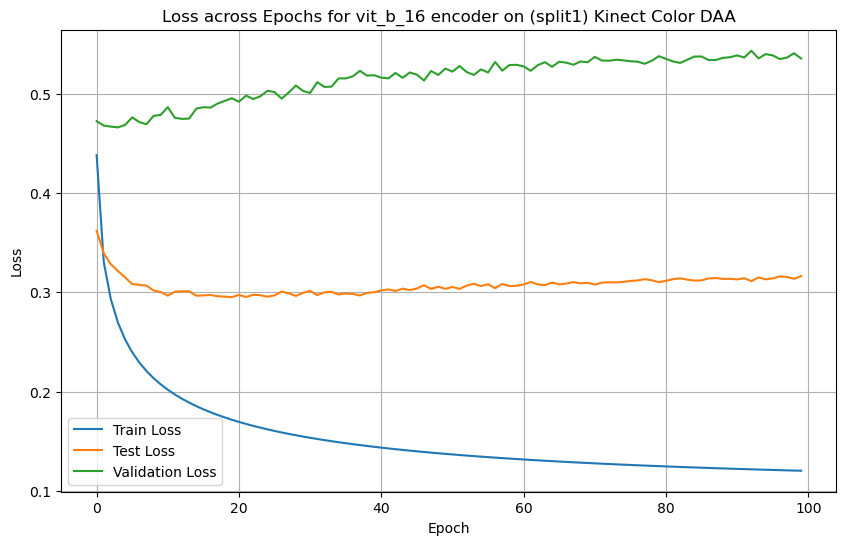
\includegraphics[width=\textwidth]{Images_Thesis/Tensboard_runs_images_all/Experiment_01_Sup_D_A_with_Aug/Split_1/output_loss_split_1_with_aug_d_a.png}
        \caption{Split 1:  Loss vs Epochs}
        \label{fig:Exp_2_04}
    \end{subfigure}

    % Third row
    \begin{subfigure}[b]{0.45\textwidth}
        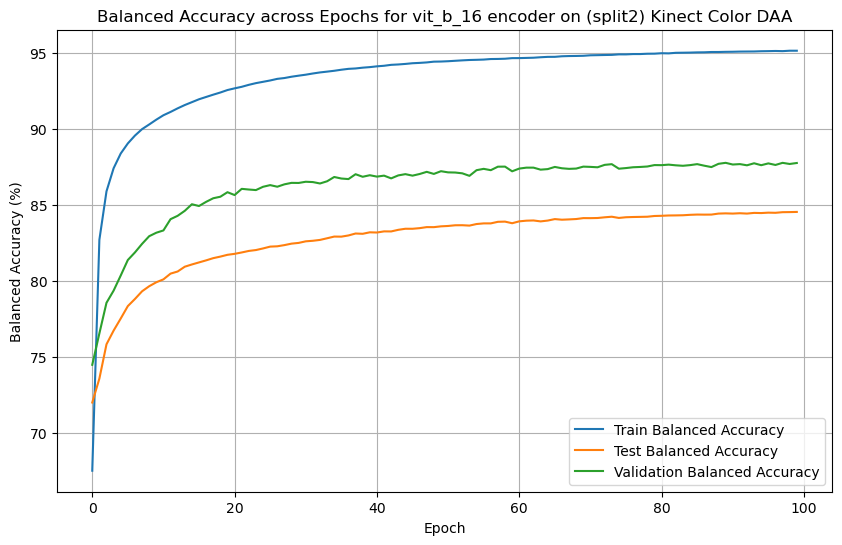
\includegraphics[width=\textwidth]{Images_Thesis/Tensboard_runs_images_all/Experiment_01_Sup_D_A_with_Aug/Split_2/output_bal_acc_split_2_with_aug_d_a.png}
        \caption{Split 2: Balanced Accuracy vs Epochs}
        \label{fig:Exp_2_05}
    \end{subfigure}
    \hfill
    \begin{subfigure}[b]{0.45\textwidth}
        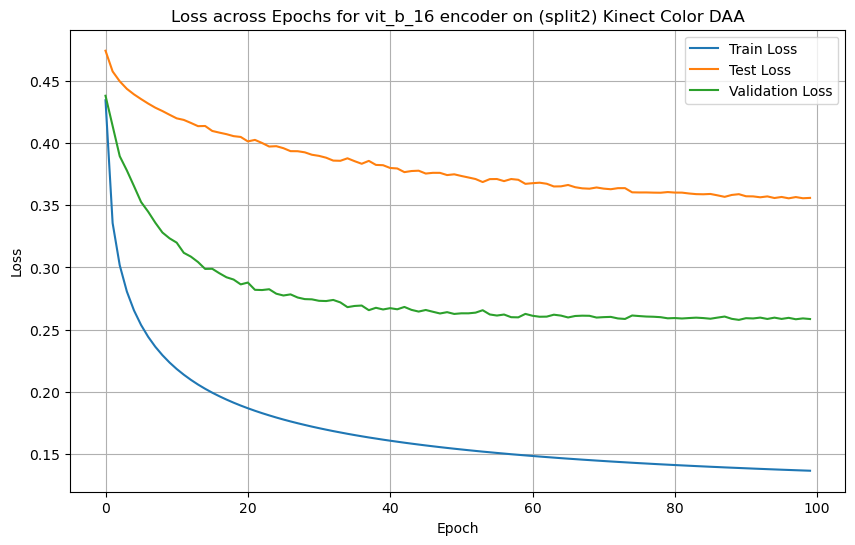
\includegraphics[width=\textwidth]{Images_Thesis/Tensboard_runs_images_all/Experiment_01_Sup_D_A_with_Aug/Split_2/output_loss_split_2_with_aug_d_a.png}
        \caption{Split 2: Loss vs Epochs}
        \label{fig:Exp_2_06}
    \end{subfigure}
    \caption[Results of Experiment 2: Supervised Learning Based Encoder with Gray Scale Augmentation]{Comparison of training and evaluation based on balanced accuracy an loss curves plotted across epochs for all three splits of Kinect Color Right Top view DAA Image dataset for supervised learning based encoder  with Gray Scale Augmentation in experiment 2.}
    \label{fig:Exp_2_00}
\end{figure}

Figure~\ref{fig:Exp_2_00} depicts the balanced accuracy and loss curves from this experiment. The figure shows that each split demonstrates high initial training balanced accuracies before shortly plateauing. This behavior highlights the effective exploitation of the pre-trained features of the vit\_b\_16 encoder, which can quickly adjust to the augmented training data. However, the validation and test accuracies throughout the splits exhibit different patterns. Split 1 test-balanced accuracy tends to stabilize at a greater level than validation.
On the contrary, for split 2, validation-balanced accuracy stabilizes at a higher level than the test. For split 1, both validation and test-balanced accuracies show a decreasing trend, which indicates overfitting. Notably, Split 2 shows better convergence for validation and test-balanced accuracies, indicating more effective generalization compared to splits 0 and 1.

The loss curves in Figure~\ref{fig:Exp_2_00} show sharp early drops in training loss in all splits, indicating efficient error minimization on the augmented grayscale training data. However, the validation loss (green) behaviors differ, with Split 1 showing an increasing trend from the start, indicating potential overfitting. On the other hand, for split 1, the test loss (orange) curve is much better and much closer to the train loss curve than the validation loss curve. In the split 0 loss curve plot, the test loss curve increases after the first few epochs, indicating poor generalization, as shown in the split 0 balanced accuracy plot. 


Like the last, this experiment evaluates the model trained on a grayscale augmented Kinect Color Right Top DAA image dataset across cross-modality and views. The data sets utilized for this evaluation are identical to those used in previous experiment. Tables \ref{table:experiment 2 results Cross Modality Generalisation} and \ref{table:experiment 2 results Cross Modality and view Generalisation on NIR} demonstrate the model's performance on the Kinect IR and NIR DAA image datasets. 
%%% Cross Modality Generalisation Tables %%%%%%%%%%
\begin{table}[htbp]
\caption{Results of Experiment 2 for Cross Modality Generalisation on test sets of Kinect IR DAA Image Dataset}
\label{table:experiment 2 results Cross Modality Generalisation}
\centering
\begin{tabular}{lllll}
\multicolumn{1}{c}{\textbf{Splits}} & \multicolumn{1}{c}{\textbf{View}} & \multicolumn{1}{c}{\textbf{Encoder}} & \multicolumn{1}{c}{\textbf{Checkpoint}} & \multicolumn{1}{c}{\textbf{Test}}\\
\hline
Split\_0 & Right Top & vit\_b\_16 & 100 & 50.58\% \\
Split\_1 & Right Top & vit\_b\_16 & 100 & 53.34\% \\
Split\_2 & Right Top & vit\_b\_16 & 100 & 60.66\% \\
\hline
Average & KIR Right Top & vit\_b\_16 & 100 & 54.86\% \\
\hline
\end{tabular}
\end{table}

%%% Cross Modality & Cross View Generalisation Tables %%%%%%%%%%
\begin{table}[htbp]
\caption{Results of Experiment 2 for Cross Modality and Cross view Generalisation on test sets of NIR DAA Image Dataset}
\label{table:experiment 2 results Cross Modality and view Generalisation on NIR}
\centering
\begin{tabular}{lllll}
\multicolumn{1}{c}{\textbf{Splits}} & \multicolumn{1}{c}{\textbf{View}} & \multicolumn{1}{c}{\textbf{Encoder}} & \multicolumn{1}{c}{\textbf{Checkpoint}} & \multicolumn{1}{c}{\textbf{Test}}\\
\hline
Split\_0 & Front Top & vit\_b\_16 & 100 & 49.68\% \\
Split\_1 & Front Top & vit\_b\_16 & 100 & 49.97\% \\
Split\_2 & Front Top & vit\_b\_16 & 100 & 49.17\% \\
\hline
Average & NIR Front Top & vit\_b\_16 & 100 & 49.60\% \\
\hline
\end{tabular}
\end{table}

\textbf{Cross-modality and cross-view generalization:}
The performance on the Kinect IR Right Top view dataset (Table \ref{table:experiment 2 results Cross Modality Generalisation}) shows that the model achieves an average test balanced accuracy of 54.86\%. This result is considerably lower than the train and test balanced accuracies observed on the augmented Kinect Color DAA dataset. However, compared to the cross-modality generalization results from experiment 1 on the Kinect IR Right Top dataset, there is an increment of 1.46\% from 53.40\% to 54.86\%. This slight increment highlights the model's challenges in generalizing to grayscale IR images. Individual splits show variability, with the highest being 60.66\% in Split 2 and the lowest at 50.58\% in Split 0, suggesting some inconsistency in the model's performance across different segments of the Kinect IR dataset.

The NIR Front Top view dataset (Table \ref{table:experiment 2 results Cross Modality and view Generalisation on NIR}) demonstrates consistent results with test balanced accuracies around 49\%. The average balanced accuracy across splits is 49.60\%, somewhat higher than experiment 1 findings on the NIR Front top view DAA dataset. This finding suggests that cross-view generalization remains challenging when the model faces a new viewing angle, stressing the relevance of the learnt features in the pre-trained encoders to the training conditions.
This also emphasizes the importance of a foundational vision model for such complicated generalization tasks, which leads this thesis to encoders trained utilizing self-supervised learning approaches on huge curated datasets without labels, as done in the~\citep{dinov2_oquab2023dinov2}.
%%%%%%%%%%%%%%%%%%%%%%%%%%%%%%%%%%%%%%%%%%%%%%%%%%%%%%%%%%%%%%
\subsection{Results of Experiment 3: Self-Supervised Learning Based Encoder}
%%%%%%%%%%%%%%%%%%%%%%%%%Text Here%%%%%%%%%%%%%%%%%%%%%%%%%%%%
As demonstrated by the results of experiment 2, by providing prior knowledge about the modality, such as augmenting color images to grayscale prior to model training, we can progress toward increasing cross-modality generalization to some extent; however, cross-view generalization still requires a robust encoder whose knowledge can be transferred to the cross-view generalization. Following the methodology in section~\ref{section:Methodology Experiment 3: Self-Supervised Learning Based Encoder}, in this experiment, we have replaced the supervised encoder with the self-supervised encoder (vit\_b\_14), which is trained using the DINOv2~\citep{dinov2_oquab2023dinov2} self-supervised learning approach on a huge curated dataset LVD-142M~\citep{dinov2_oquab2023dinov2} with 142 million images without labels. This experiment's setup is identical to that of experiment 1, using the same hyperparameters to provide a fair performance comparison.

%%%%%%%%%%%%%%%%%% Grid of class distributions %%%%%%%%%%%%%%%%%
\begin{figure}[htbp]
    \centering
    % First row
    \begin{subfigure}[b]{0.45\textwidth}
        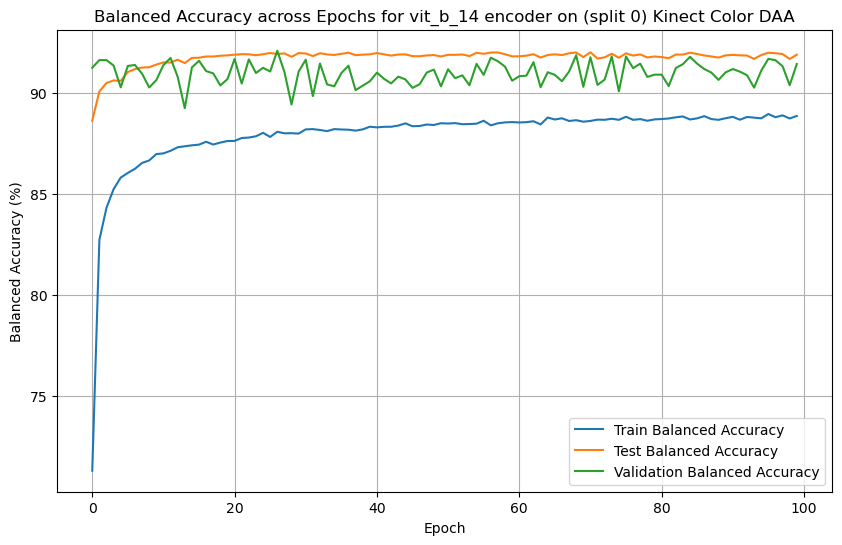
\includegraphics[width=\textwidth]{Images_Thesis/Tensboard_runs_images_all/Experiment_02_Sel_Sup_D_A_no_Aug/Split_0/output_bal_acc_split_0_d_a_ssl.png}
        \caption{Split 0: Balanced Accuracy vs Epochs}
        \label{fig:Exp_3_01}
    \end{subfigure}
    \hfill % space between images
    \begin{subfigure}[b]{0.45\textwidth}
        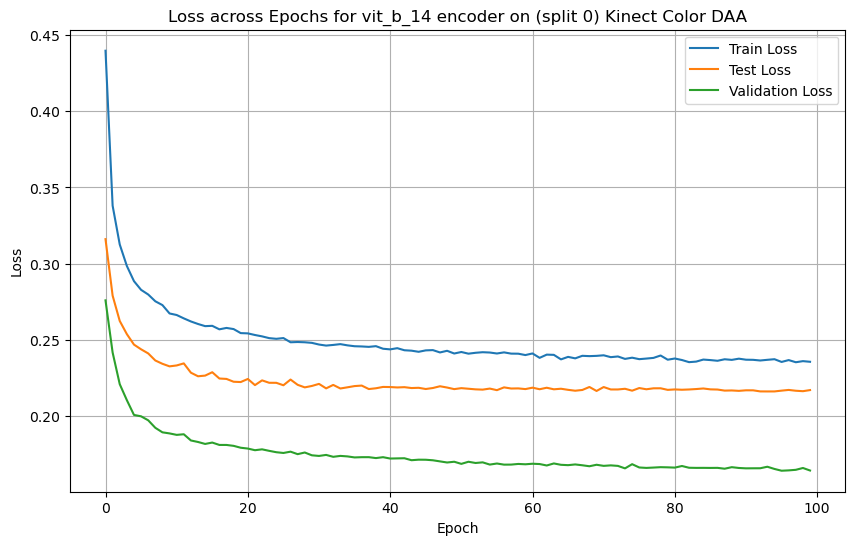
\includegraphics[width=\textwidth]{Images_Thesis/Tensboard_runs_images_all/Experiment_02_Sel_Sup_D_A_no_Aug/Split_0/output_loss_split_0_d_a_ssl.png}
        \caption{Split 0: Loss vs Epochs}
        \label{fig:Exp_3_02}
    \end{subfigure}

    % Second row
    \begin{subfigure}[b]{0.45\textwidth}
        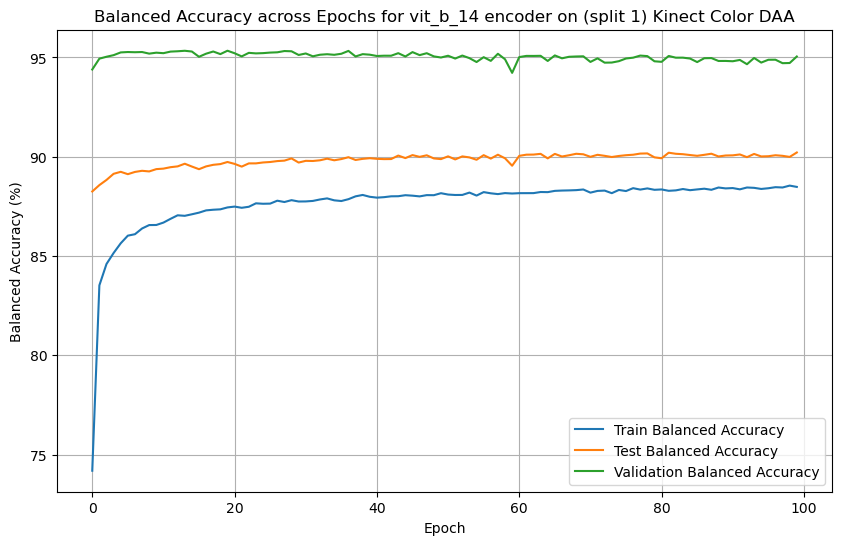
\includegraphics[width=\textwidth]{Images_Thesis/Tensboard_runs_images_all/Experiment_02_Sel_Sup_D_A_no_Aug/Split_1/output_bal_acc_split_1_d_a_ssl.png}
        \caption{Split 1: Balanced Accuracy vs Epochs}
        \label{fig:Exp_3_03}
    \end{subfigure}
    \hfill
    \begin{subfigure}[b]{0.45\textwidth}
        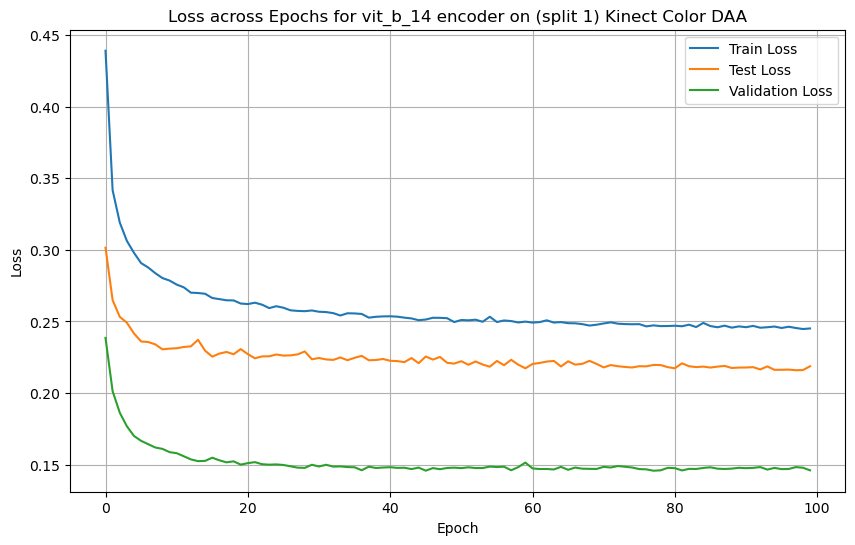
\includegraphics[width=\textwidth]{Images_Thesis/Tensboard_runs_images_all/Experiment_02_Sel_Sup_D_A_no_Aug/Split_1/output_loss_split_1_d_a_ssl.png}
        \caption{Split 1:  Loss vs Epochs}
        \label{fig:Exp_3_04}
    \end{subfigure}

    % Third row
    \begin{subfigure}[b]{0.45\textwidth}
        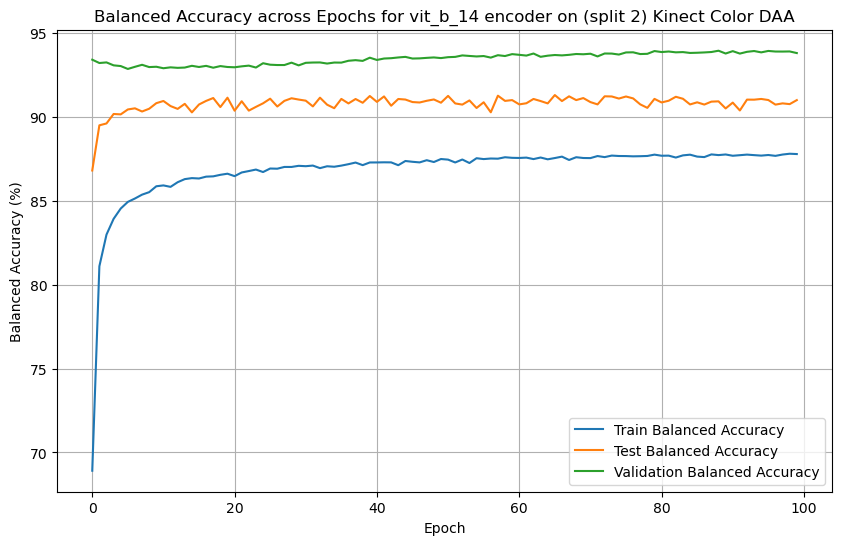
\includegraphics[width=\textwidth]{Images_Thesis/Tensboard_runs_images_all/Experiment_02_Sel_Sup_D_A_no_Aug/Split_2/output_bal_acc_split_2_d_a_ssl.png}
        \caption{Split 2: Balanced Accuracy vs Epochs}
        \label{fig:Exp_3_05}
    \end{subfigure}
    \hfill
    \begin{subfigure}[b]{0.45\textwidth}
        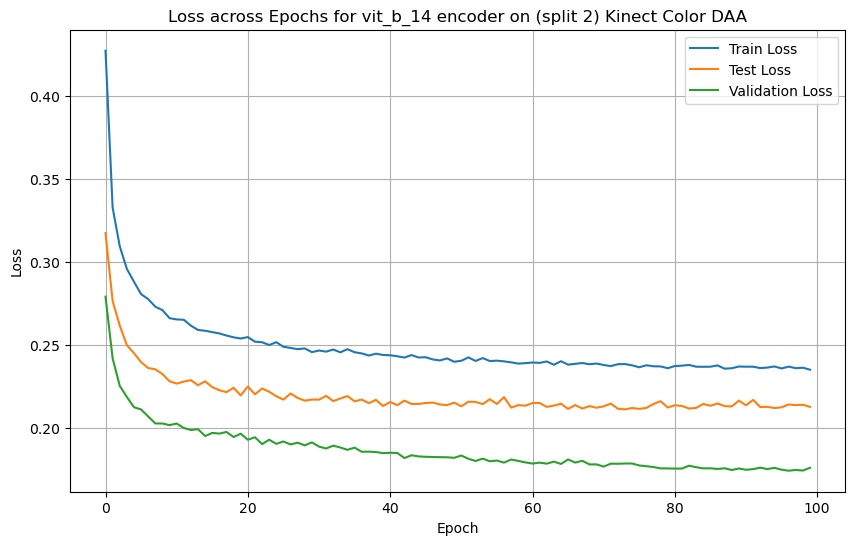
\includegraphics[width=\textwidth]{Images_Thesis/Tensboard_runs_images_all/Experiment_02_Sel_Sup_D_A_no_Aug/Split_2/output_loss_split_2_d_a_ssl.png}
        \caption{Split 2: Loss vs Epochs}
        \label{fig:Exp_3_06}
    \end{subfigure}
    \caption[Results of Experiment 3: Self Supervised Learning Based Encoder]{Comparison of training and evaluation based on balanced accuracy an loss curves plotted across epochs for all three splits of Kinect Color Right Top view DAA Image dataset for self supervised learning based encoder in experiment 3.}
    \label{fig:Exp_3_00}
\end{figure}

Table~\ref{table:experiment 3 results} shows an average training balanced accuracy of 88.36\% across all splits, indicating the model's strong capacity to learn from Kinect Right Top view color training data. However, the validation balanced accuracies are significantly higher, averaging 93.42 percent, indicating underfitting. The average test-balanced accuracy is slightly lower than validation-balanced accuracy at 91.02\%, demonstrating a decent generalization to unseen data.
%%%%%%%%%%%% Result table: Experiment 3 %%%%%%%%%%%
\begin{table}[htbp]
\caption{Results of Experiment 3: Self-Supervised Learning Based Encoder}
\label{table:experiment 3 results}
\centering
\begin{tabular}{llllll}
\multicolumn{1}{c}{\textbf{Splits}} & \multicolumn{1}{c}{\textbf{View}} & \multicolumn{1}{c}{\textbf{Encoder}} & \multicolumn{1}{c}{\textbf{Train}} & \multicolumn{1}{c}{\textbf{Val}} & \multicolumn{1}{c}{\textbf{Test}}\\
\hline
Split\_0 & Right Top & DINOv2\_vit\_b\_14 & 88.83\% & 91.41\% & 91.87\% \\
Split\_1 & Right Top & DINOv2\_vit\_b\_14 & 88.48\% & 95.04\% & 90.21\% \\
Split\_2 & Right Top & DINOv2\_vit\_b\_14 & 87.79\% & 93.81\% & 91.00\% \\
\hline
Average & Right Top & DINOv2\_vit\_b\_14 & 88.36\% & 93.42\% & 91.02\% \\
\hline
\end{tabular}
\end{table}

Validation-balanced accuracies are much higher than training-balanced accuracies, indicating that the model trained using Kinect color right top view dataset generalizes across the dataset well. Similarly, the test-balanced accuracy also supports this argument by showing higher test-balanced accuracies than the training-balanced accuracies across all splits for the Kinect color right top view dataset. Figure~\ref{fig:Exp_3_00} depicts the balanced accuracy and loss curves from this experiment. The figure shows that each split demonstrates high initial validation and test balanced accuracies before shortly plateauing. 

The train balanced accuracy curves in the figure~\ref{fig:Exp_3_00} for all three splits reveals that although the model is underfitting, there is a lot higher generalization on unseen test data than in the prior two experiments. This demonstrates the robustness and powerful features that the DINOv2-based vit\_b\_14 encoder has. The loss curves in the figure~\ref{fig:Exp_3_00} also support the underfitting on all three splits. This suggests the need for different hyperparameter configurations for this experiment, which contributes to the future scope of this thesis.

Similar to the earlier two experiments, this experiment evaluates the model trained on a Kinect Color Right Top view DAA image dataset across cross-modality and views. The data sets utilized for this evaluation are identical to those used in earlier two experiments. Tables \ref{table:experiment 3 results Cross Modality Generalisation} and \ref{table:experiment 3 results Cross Modality and view Generalisation on NIR} demonstrate the model's performance on the Kinect IR and NIR DAA image datasets.

\textbf{Cross-Modality and Cross-View Generalization:}
The performance on the Kinect IR Right Top view dataset (Table \ref{table:experiment 3 results Cross Modality Generalisation}) shows that the model achieves an average test balanced accuracy of 60.57\%. This result is considerably lower than the test balanced accuracies observed on the Kinect Color Right Top view DAA dataset. However, compared to the cross-modality generalization results from experiment 1 and experiment 2 on the Kinect IR Right Top view dataset, there is an increment of 7.17\% from 53.40\% in experiment to 60.57\% in experiment 3 and 5.71\% from 54.86\% in experiment 1 to 60.57\% in experiment 3. This shows the superiority of the self-supervised learning-based encoder over the supervised learning-based encoder under consideration in this thesis on cross-modality generalization.
%%%%%%%%%%%%%%%%%%%%%%%%%%%%%%%%%%%%%%%%%%%%%%%%%%%%%%%%%%%%%%
%%% Cross Modality Generalisation Tables %%%%%%%%%%
\begin{table}[htbp]
\caption{Results of Experiment 3 for Cross Modality Generalisation on test sets of Kinect IR DAA Image Dataset}
\label{table:experiment 3 results Cross Modality Generalisation}
\centering
\begin{tabular}{lllll}
\multicolumn{1}{c}{\textbf{Splits}} & \multicolumn{1}{c}{\textbf{View}} & \multicolumn{1}{c}{\textbf{Encoder}} & \multicolumn{1}{c}{\textbf{Checkpoint}} & \multicolumn{1}{c}{\textbf{Test}}\\
\hline
Split\_0 & Right Top & DINOv2\_vit\_b\_14 & 100 & 71.80\% \\
Split\_1 & Right Top & DINOv2\_vit\_b\_14 & 100 & 56.64\% \\
Split\_2 & Right Top & DINOv2\_vit\_b\_14 & 100 & 53.27\% \\
\hline
Average & KIR Right Top & DINOv2\_vit\_b\_14 & 100 & 60.57\% \\
\hline
\end{tabular}
\end{table}

%%% Cross Modality & Cross View Generalisation Tables %%%%%%%%%%
\begin{table}[htbp]
\caption{Results of Experiment 3 for Cross Modality and Cross view Generalisation on test sets of NIR DAA Image Dataset}
\label{table:experiment 3 results Cross Modality and view Generalisation on NIR}
\centering
\begin{tabular}{lllll}
\multicolumn{1}{c}{\textbf{Splits}} & \multicolumn{1}{c}{\textbf{View}} & \multicolumn{1}{c}{\textbf{Encoder}} & \multicolumn{1}{c}{\textbf{Checkpoint}} & \multicolumn{1}{c}{\textbf{Test}}\\
\hline
Split\_0 & Front Top & DINOv2\_vit\_b\_14 & 100 & 50.05\% \\
Split\_1 & Front Top & DINOv2\_vit\_b\_14 & 100 & 51.10\% \\
Split\_2 & Front Top & DINOv2\_vit\_b\_14 & 100 & 50.49\% \\
\hline
Average & NIR Front Top & DINOv2\_vit\_b\_14 & 100 & 50.54\% \\
\hline
\end{tabular}
\end{table}

Further evaluating the model's generalization capabilities, the NIR Front Top view dataset (Table \ref{table:experiment 3 results Cross Modality and view Generalisation on NIR}) shows test balanced accuracies hovering around 50\%. The average balanced accuracy across the splits on the NIR Front top view DAA dataset stands at 50.54\%, which is 1.3\% greater than the one in experiment 1 and 0.94\% greater than the one in experiment 2. However, no significant improvement has been obtained, even using a very powerful encoder on cross-view and cross-modality generalization on the NIR Front Top view dataset. This shows that in order to improve the cross-view and cross-modality generalization on the NIR Front Top view dataset, the model needs prior training on the train sets of this dataset. To further enhance the performance on the NIR Front Top view dataset, the encoder can be completely fine-tuned on the datasets by unfreezing its pre-trained parameters for training, which will be computationally expensive given the large size and three splits of the \gls{daa} datasets.

\subsection{Results of Experiment 4: Self-Supervised Learning Based Encoder with Clustered Feature Weighting Data-loading}
%%%%%%%%%%%%%%%%%%%%%%%%%Text Here%%%%%%%%%%%%%%%%%%%%%%%%%%%%
In our previous three experiments, we assessed the efficacy of various training paradigms using a pre-trained vision transformer encoder obtained from supervised and self-supervised learning paradigms. The experiments examined the impact of pre-trained encoders on driver distraction detection. The datasets considered in this thesis were analyzed from a cross-modality and cross-view generalization perspective for driver distraction detection, utilizing the traditional imbalanced data-loading approach.

%%%%%%%%%%%%%%%%%% Grid of class distributions %%%%%%%%%%%%%%%%%
\begin{figure}[htbp]
    \centering
    % First row
    \begin{subfigure}[b]{0.45\textwidth}
        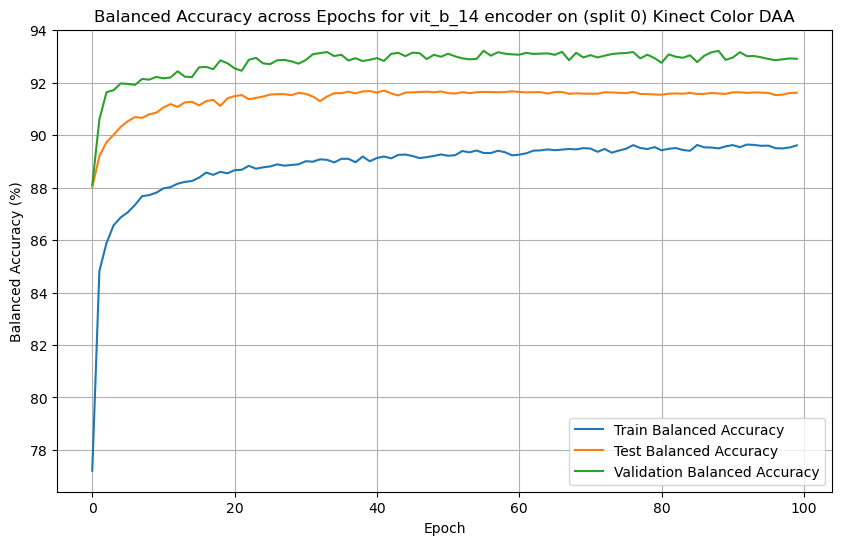
\includegraphics[width=\textwidth]{Images_Thesis/Tensboard_runs_images_all/Experiment_03_Sel_Sup_D_B_no_Aug/Split_0/output_bal_acc_split_0_d_b_ssl.png}
        \caption{Split 0: Balanced Accuracy vs Epochs}
        \label{fig:Exp_4_01}
    \end{subfigure}
    \hfill % space between images
    \begin{subfigure}[b]{0.45\textwidth}
        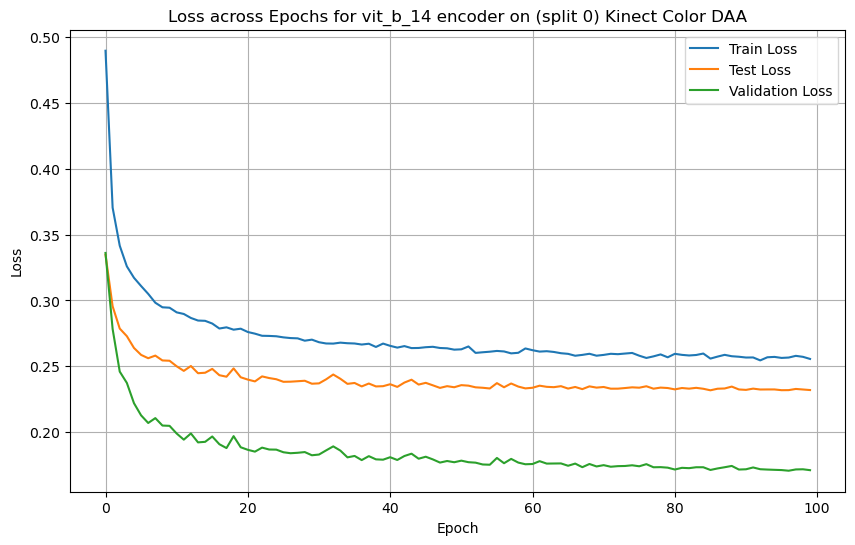
\includegraphics[width=\textwidth]{Images_Thesis/Tensboard_runs_images_all/Experiment_03_Sel_Sup_D_B_no_Aug/Split_0/output_loss_split_0_d_b_ssl.png}
        \caption{Split 0: Loss vs Epochs}
        \label{fig:Exp_4_02}
    \end{subfigure}

    % Second row
    \begin{subfigure}[b]{0.45\textwidth}
        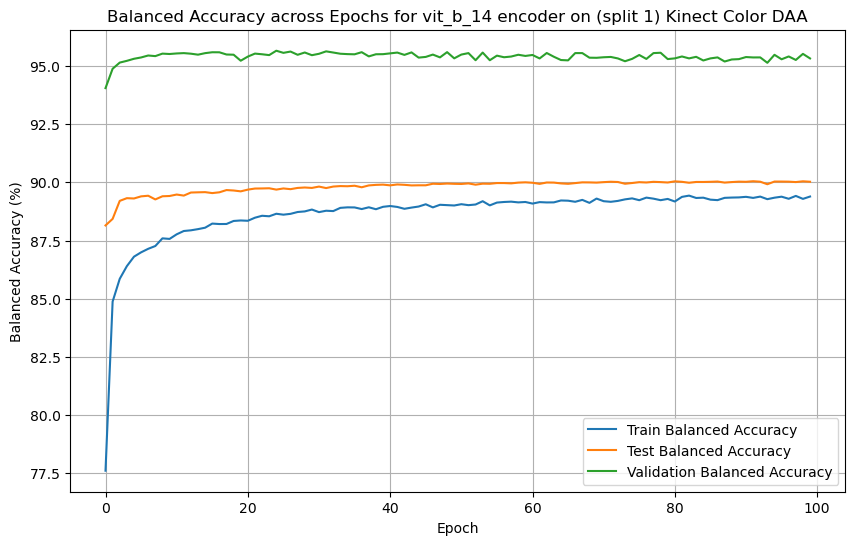
\includegraphics[width=\textwidth]{Images_Thesis/Tensboard_runs_images_all/Experiment_03_Sel_Sup_D_B_no_Aug/Split_1/output_bal_acc_split_1_d_b_ssl.png}
        \caption{Split 1: Balanced Accuracy vs Epochs}
        \label{fig:Exp_4_03}
    \end{subfigure}
    \hfill
    \begin{subfigure}[b]{0.45\textwidth}
        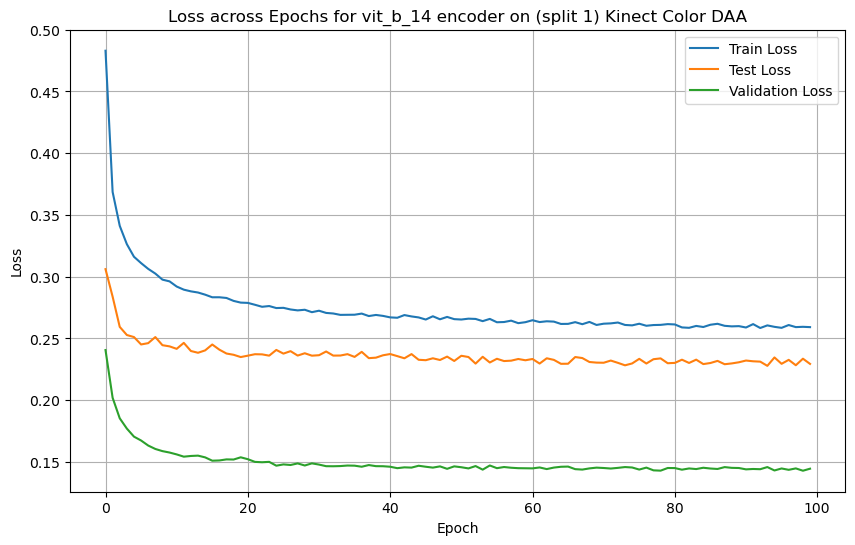
\includegraphics[width=\textwidth]{Images_Thesis/Tensboard_runs_images_all/Experiment_03_Sel_Sup_D_B_no_Aug/Split_1/output_loss_split_1_d_b_ssl.png}
        \caption{Split 1:  Loss vs Epochs}
        \label{fig:Exp_4_04}
    \end{subfigure}

    % Third row
    \begin{subfigure}[b]{0.45\textwidth}
        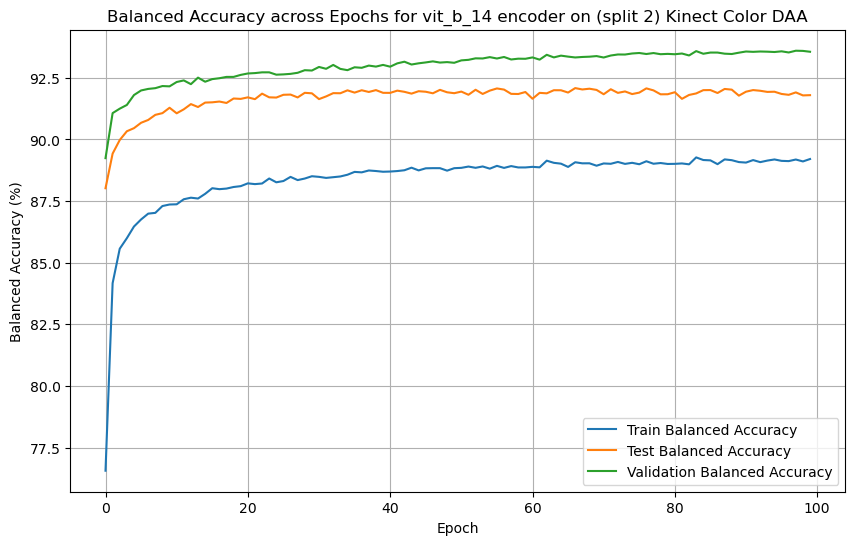
\includegraphics[width=\textwidth]{Images_Thesis/Tensboard_runs_images_all/Experiment_03_Sel_Sup_D_B_no_Aug/Split_2/output_bal_acc_split_2_d_b_ssl.png}
        \caption{Split 2: Balanced Accuracy vs Epochs}
        \label{fig:Exp_4_05}
    \end{subfigure}
    \hfill
    \begin{subfigure}[b]{0.45\textwidth}
        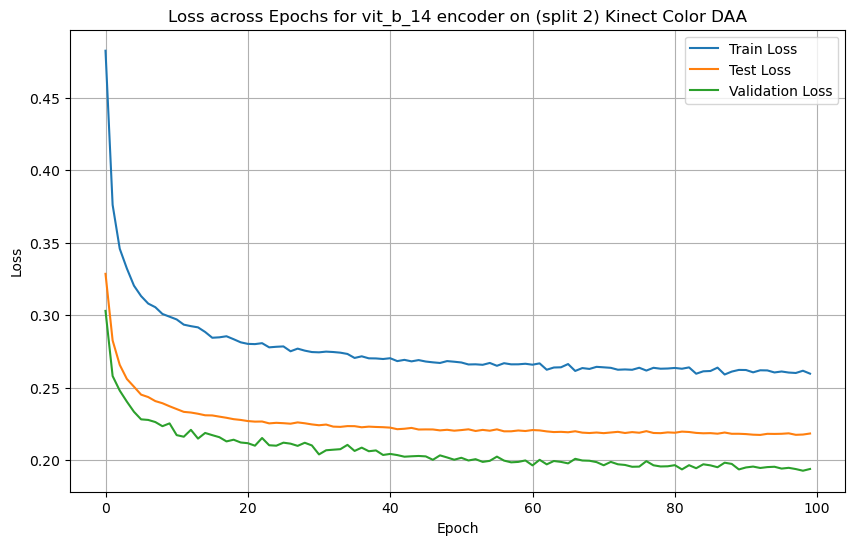
\includegraphics[width=\textwidth]{Images_Thesis/Tensboard_runs_images_all/Experiment_03_Sel_Sup_D_B_no_Aug/Split_2/output_loss_split_2_d_b_ssl.png}
        \caption{Split 2: Loss vs Epochs}
        \label{fig:Exp_4_06}
    \end{subfigure}
    \caption[Results of Experiment 4: Self Supervised Learning Based Encoder with Clustered Feature Weighting Data-loading]{Comparison of training and evaluation based on balanced accuracy an loss curves plotted across epochs for all three splits of Kinect Color Right Top view DAA Image dataset for self supervised learning based encoder with Clustered Feature Weighting Data-loading in experiment 4.}
    \label{fig:Exp_4_00}
\end{figure}

Nevertheless, this thesis suggests a data loading approach called ``Clustered Feature Weighting" to enhance the imbalance in loading data in batches. This experiment evaluates the impact of modifying the dataloading strategy on driver distraction detection performance. Specifically, it focuses on three aspects: the driver distraction detection performance on the Kinect Color Right Top view DAA image dataset, the cross-modality generalization for driver distraction detection on the Kinect IR Right Top view DAA image dataset, and the cross-view and cross-modality generalization for driver distraction detection on the NIR Front Top-view DAA image dataset.

So, following the methodology in section~\ref{section: Methodology Experiment 4: Self-Supervised Learning Based Encoder with Clustered Feature Weighting Data-loading}, we have used clustered feature data loading with the self-supervised encoder (vit\_b\_14) in this experiment. This experiment's setup is identical to that of experiment 1, using the same hyperparameters to provide a fair performance comparison.
%%%%%%%%%%%% Result table: Experiment 4 %%%%%%%%%%%
\begin{table}[htbp]
\caption{Results of Experiment 4: Self-Supervised Learning Based Encoder with Clustered Feature Weighting Data-loading}
\label{table:experiment 4 results}
\centering
\begin{tabular}{llllll}
\multicolumn{1}{c}{\textbf{Splits}} & \multicolumn{1}{c}{\textbf{View}} & \multicolumn{1}{c}{\textbf{Encoder}} & \multicolumn{1}{c}{\textbf{Train}} & \multicolumn{1}{c}{\textbf{Val}} & \multicolumn{1}{c}{\textbf{Test}}\\
\hline
Split\_0 & Right Top & DINOv2\_vit\_b\_14 & 89.61\% & 92.91\% & 91.62\% \\
Split\_1 & Right Top & DINOv2\_vit\_b\_14 & 89.38\% & 95.32\% & 90.02\% \\
Split\_2 & Right Top & DINOv2\_vit\_b\_14 & 89.20\% & 93.55\% & 91.79\% \\
\hline
Average & Right Top & DINOv2\_vit\_b\_14 & 89.39\% & 93.92\% & 91.14\% \\
\hline
\end{tabular}
\end{table}

Table~\ref{table:experiment 4 results} shows driver distraction detection performance on the Kinect Color Right Top view dataset with an average training balanced accuracy of 89.39\% across all splits with an improvement of 1.03\% from experiment 3.The validation balanced accuracies average 93.92 percent,  indicating underfitting using novel data-loading, too. The balanced accuracy and loss curves in figure~\ref{fig:Exp_4_00} further confirm the phenomenon of underfitting. The average test-balanced accuracy is slightly lower than validation-balanced accuracy at 91.14\%, demonstrating a decent generalization to unseen test set data of Kinect Color dataset. In comparison to experiment 3, the train balanced accuracy in this experiment on the Kinect Color Right Top view dataset is 1.03\% higher. Additionally, the validation balanced accuracy is 0.5\% higher, and the test balanced accuracy is 0.08\% higher than in experiment 3. These results indicate that the model requires different hyperparameter configuration to prevent underfitting and assess the overall effectiveness and limitations of the `Clustered Feature Weighting' data-loading technique on the model's performance on driver distraction detection task.    

\textbf{Cross-Modality and Cross-View Generalization:}
The performance on the Kinect IR Right Top view dataset (Table \ref{table:experiment 4 results Cross Modality Generalisation}) shows that the model achieves an average test balanced accuracy of 54.37\%. 
%%% Cross Modality Generalisation Tables %%%%%%%%%%
\begin{table}[htbp]
\caption{Results of Experiment 4 for Cross Modality Generalization on test sets of Kinect IR DAA Image Dataset}
\label{table:experiment 4 results Cross Modality Generalisation}
\centering
\begin{tabular}{lllll}
\multicolumn{1}{c}{\textbf{Splits}} & \multicolumn{1}{c}{\textbf{View}} & \multicolumn{1}{c}{\textbf{Encoder}} & \multicolumn{1}{c}{\textbf{Checkpoint}} & \multicolumn{1}{c}{\textbf{Test}}\\
\hline
Split\_0 & Right Top & DINOv2\_vit\_b\_14 & 100 & 59.57\% \\
Split\_1 & Right Top & DINOv2\_vit\_b\_14 & 100 & 52.75\% \\
Split\_2 & Right Top & DINOv2\_vit\_b\_14 & 100 & 50.81\% \\
\hline
Average & KIR Right Top & DINOv2\_vit\_b\_14 & 100 & 54.37\% \\
\hline
\end{tabular}
\end{table}

%%% Cross Modality & Cross View Generalisation Tables %%%%%%%%%%
\begin{table}[htbp]
\caption{Results of Experiment 4 for Cross Modality and Cross view Generalization on test sets of NIR DAA Image Dataset}
\label{table:experiment 4 results Cross Modality and view Generalisation on NIR}
\centering
\begin{tabular}{lllll}
\multicolumn{1}{c}{\textbf{Splits}} & \multicolumn{1}{c}{\textbf{View}} & \multicolumn{1}{c}{\textbf{Encoder}} & \multicolumn{1}{c}{\textbf{Checkpoint}} & \multicolumn{1}{c}{\textbf{Test}}\\
\hline
Split\_0 & Front Top & DINOv2\_vit\_b\_14 & 100 & 50.05\% \\
Split\_1 & Front Top & DINOv2\_vit\_b\_14 & 100 & 51.00\% \\
Split\_2 & Front Top & DINOv2\_vit\_b\_14 & 100 & 50.69\% \\
\hline
Average & NIR Front Top & DINOv2\_vit\_b\_14 & 100 & 50.58\% \\
\hline
\end{tabular}
\end{table}
The results from the Kinect IR Right Top view dataset (Table \ref{table:experiment 4 results Cross Modality Generalisation}) indicate that the model attains an average test balanced accuracy of 54.37\%. 
Upon further evaluation of the model's ability to generalize, the NIR Front Top view dataset (Table \ref{table:experiment 4 results Cross Modality and view Generalisation on NIR}) demonstrates an average test balanced accuracy of 50.58\% across the splits on the NIR Front top view DAA dataset. This accuracy is 1.34\% higher than that of experiment 1, 0.98\% higher than that of experiment 2, and 0.08\% higher than that of experiment 3. Despite using a powerful encoder and balanced data-loading, there has been no notable increase in comparison to experiment 3 in terms of cross-view and cross-modality generalization on the NIR Front Top view dataset. This demonstrates that, in order to improve the ability to generalize across multiple views and modality in the NIR Front Top view dataset, the problem of underfitting must be addressed. Furthermore, the model must be pre-trained using the training sets from this dataset, as previously described in experiment 3.

\section{Answers to Research Questions}
\label{section:answers_to_research_questions}
This section provides detailed answers based on the experimental findings for the central research questions guiding this thesis.

\subsection{Practical Challenges}
The issue of data imbalance in the \gls{daa} dataset was effectively addressed by employing the novel `Clustered Feature Weighting' dataloading technique. This technique leverages unsupervised learning, specifically using the HDBSCAN algorithm for clustering based on features extracted by a pretrained vision transformer. The inclusion of a weighted random sampler resulted in balanced batches, indicating consistent training and indications of improvement in the performance of the deep learning models.

\subsection{Effectiveness of SSL Models}
The use of vision transformer encoders pretrained with the \gls{ssl} method, specifically DINOv2~\citep{dinov2_oquab2023dinov2}, showed significant benefits in detecting driver distraction. These encoders provided robust feature extraction capabilities, which improved generalization over the supervised learning encoder. The main drawback observed was a slight underfitting in the fixed experimental setup, suggesting that these models might require further tuning of hyperparameters or training procedures to fully capitalize on their potential.

\subsection{Generalization Capabilities}
The different image views, namely the right top view and the front top view from the \gls{daa} dataset, demonstrated that the vision transformer encoder pretrained using the \gls{ssl} approach maintains a relatively consistent performance on driver distraction detection task. However, generalization across these views was not completely uniform, indicating that while the \gls{ssl} models can handle view variability to a certain extent, there is still room for improvement in model training or architecture to enhance view-invariant feature extraction.

\subsection{Data Modality Impact}
The impact of varying data modalities, such as RGB and infrared (IR) images, was significant on the detection of driver distractions. The DINOv2~\citep{dinov2_oquab2023dinov2} pretrained vision transformer encoder exhibited better generalization across these modalities compared to models trained with supervised learning approaches. Although the performance on NIR datasets was less impressive, it still marked an improvement over traditional models, emphasizing the potential of \gls{ssl} models in handling diverse input types. This suggests a promising direction for future research in using self-supervised learning to develop more adaptable and effective driver distraction detection systems.

